%#####################################################################
%                            Document
%#####################################################################

%#####################################################################
%                            LaTeX starts
%#####################################################################


\documentclass[draft=false,           % draft modus (true,false)
               paper=a4,              % paper size  (print space)
               fontsize=11pt,         % font size (10pt,11pt,12pt)
               headings=big,
               twocolumn=false,       % text columns per page (true,false)
               twoside,               % text side layout (oneside,twoside)
               openright,             % start chapter (openright,openany)
               chapterprefix,         % two lines chapters 'Chapter x\\ Name'
               cleardoublepage=plain, % new (twoside) page (empty,plain,standard)
               parskip=false,
               numbers=noenddot        % configure \parindent and \parskip
              ]{scrbook}

%\documentclass[a4paper,12pt,twoside,openany,headsepline,bibliography=totocnumbered]{scrbook}

%%% HAS TO BE HERE FOR TIKZ %%%
\usepackage{etex}

% *************************************************************

% packages (really needed ones only)
%% A
\usepackage[printonlyused]{acronym}          	% abbreviations
\usepackage{adjustbox}                       	
\usepackage{algorithm}                       	% algorithms
\usepackage{algpseudocode}                     % algorithms
\usepackage{amssymb}                          % misc extra (math) symbols
\usepackage{amsthm}
%% B
\usepackage[ngerman,american]{babel}          % US English terms and hyphenations
\usepackage{booktabs}													% Nice table stuff like \toprule
%% C
\usepackage{color}
\usepackage{colortbl}
%% D
%% E
\usepackage{enumitem}												  % Control over lists
\usepackage{extarrows}												% Long arrows
%% F
\usepackage{fancyhdr}                         % custom headers & footers
\usepackage{float}
\usepackage{footmisc}													% Labels in footnotes
%\usepackage[T1]{fontenc}                      % force T1 vector font encoding
\usepackage{framed}
\usepackage[in,headings]{fullpage}            % 1 inch margins, header & footers, centering
%% G
\usepackage{graphicx}                  				% graphic stuff
%% H
\usepackage{here}
\usepackage[pdftitle={David Oswald -- Hardware and Embedded Systems Security},pdfsubject={Hardware and Embedded Systems Security}, pdfauthor={David Oswald}, pdfkeywords={Keywords}, pdfdisplaydoctitle=true, linktocpage=true, bookmarksnumbered=true, colorlinks=false, linkcolor=blue, citecolor=blue, anchorcolor=blue, pdfpagelayout=TwoPageRight, bookmarksopen=true, bookmarksopenlevel=0]{hyperref}
%% I
\usepackage[utf8]{inputenc}                 % allow direct input of umlaute etc.
%% J
%% K
%% L
% \usepackage{l3backend} 
\usepackage{listings}                         % sophisticated source code listings
\usepackage{lmodern}													% better fonts
\usepackage{longtable}                        % multi-page tables
%% M
\usepackage{makeidx}                          % enable indexing (cf. \makeindex)
%\usepackage[k-loose,nohints]{minitoc}         % mini tocs per chapter
\usepackage{multirow}													% For multiple rows in tables
%% N
\usepackage{nopageno}                         % disable auto page numbering
\usepackage{nicefrac}													% smaller fraction symbol
%% O
%% P
\usepackage{placeins}													% for \FloatBarrier
\usepackage{protocol}													% for typesetting protocols
\usepackage{pstricks}
\usepackage{pst-all}
%% Q
%% R
%% S
\usepackage{subfig}														% For \subfloat
%% T
\usepackage{tabularx}													% Better tables
\usepackage{textcomp}													% Fix pound problem
\usepackage{tikz}                             % Drawings
%% U
\usepackage{upgreek}													% ``Unmathematical'' greek symbols eg. for units
\usepackage{url}                              % URL handling (style & line breaks)
%% V
%% W
%% X
%% Y
%% Z

%%% Need all libs here
\usetikzlibrary{shapes,arrows,calc}
\usetikzlibrary{shapes}
\usetikzlibrary{positioning}
\usetikzlibrary{matrix}

% Links
\hypersetup{
    colorlinks,
    linkcolor={red!30!black},
    citecolor={blue!50!black},
    urlcolor={blue!80!black}
}

%#####################################################################
%                        Layout customization
%#####################################################################

% spacing between headline and text
\setlength{\headsep}{20pt}

% line spacing (don't use \baselinestretch)
%\linespread{1.1}

% flexible extra vertical space between paragraphs (default +0.5 -0.25)
%\setlength{\parskip}{1ex plus0.5ex minus0.25ex}

% maximum fraction of a page for floats before creating a new page
\renewcommand{\floatpagefraction}{0.75} % (default = 0.5)

% minimum fraction of a page for text (default = 0.2)
%\renewcommand{\textfraction}{0.2}

% penalties to prevent 'Hurenkinder' and 'Schusterjungen'
\clubpenalty = 10000
\widowpenalty = 10000
\displaywidowpenalty = 10000

% penalty for word spacing vs. overlapping words
\tolerance = 500

% makes all text pages the same height, by adding
% extra vertical space when necessary (book default)
\flushbottom % \raggedbottom (no extra vertical space)

% center chapter headings
\addtokomafont{chapter}{\renewcommand*{\raggedsection}{\centering}}

% Try to fix PDF graphics CMYK<->RGB bug on MAC
%\pdfpageattr {/Group << /S /Transparency /I true /CS /DeviceRGB>>}

% define some own fonts
\newcommand{\subtitlefnt}{\fontfamily{ppl}\fontshape{sl}\fontseries{m}\fontsize{13}{16}\selectfont}

% define fancy page style
\pagestyle{fancy}

% define page headings
\fancyhead{} % clear previous
\fancyhead[LE]{\textsf{\nouppercase{\leftmark}}}
\fancyhead[RO]{\textsf{\nouppercase{\rightmark}}}
\renewcommand{\headrulewidth}{0.5pt}

% define page footers
\fancyfoot{} % clear previous
\fancyfoot[EL,OR]{\textsf{\thepage}}
\fancyfoot[ER,OL]{}

% define some custom colors
\definecolor{itemcolor}{rgb}{0.3,0.3,0.3}

% use different itemize bullets (first & second level)
\renewcommand{\labelitemi}{\graybox}
\renewcommand{\labelitemii}{\whitebox}

% use different enumerate  (first & second level), e.g., R/roman, Arabic,
\renewcommand{\labelenumi}{(\arabic{enumi})}
\renewcommand{\labelenumii}{\alph{enumii})}

\newtheorem{definition}{Definition}


%#####################################################################
%                Custom settings, commands & macros
%#####################################################################
% chapter introduction texts
\newcommand{\chapterintro}[1]{\begin{quote}\emph{\noindent #1}\end{quote}\medskip}

% customized paragraphs
\newcommand{\boldpar}[1]{\smallskip\noindent\textbf{#1}}
\newcommand{\italicpar}[1]{\smallskip\noindent\emph{#1}}

% command for in text comments
\newcommand{\comout}[1]{}

% customized 'mandatory' and 'optional' symbols (e.g., used in tables)
\newcommand{\mnd}{$\blacksquare$}
\newcommand{\opt}{$\square$}

% define some custom symbols
\newcommand{\graybox}{{\scriptsize\textcolor{itemcolor}{$\blacksquare$}}}
\newcommand{\halfbox}{{\normalsize\textcolor{itemcolor}{$\blacklozenge$}}}
\newcommand{\whitebox}{{\scriptsize\textcolor{itemcolor}{$\square$}}}

%% Altera
\newcommand{\eg}{e.g., }
\newcommand{\ie}{i.e., }
\newcommand{\etal}{et al. }
\newcommand{\etc}{etc.~}
\newcommand{\Sbox}{S-box}
\newcommand{\Fig}{Fig.}
\newcommand{\sxii}{Stratix~II}
\newcommand{\quar}{Quartus~II}
\newcommand{\todo}[1]{\textcolor{red}{\textsf{TODO: #1}}}

%% DESFire
\newcommand{\Ohm}{\ensuremath{\Upomega}}
\newcommand{\Reals}{\mathbb{R}}
\newcommand{\bigo}{\mathcal{O}}
\newcommand{\pbigo}[1]{\mathcal{O}\left(#1\right)}
\newcommand{\binfield}[1]{\mathbb{F}_2^{#1}}
\newcommand{\timefreq}{\circ\kern-0.4em-\kern-0.4em\bullet}
\newcommand{\degree}{\ensuremath{^\circ}}
\newcommand{\bitvec}[1]{\ensuremath{\vec{#1}}}
\newcommand{\bitget}[2]{\ensuremath{ \vec{#2}^{\left(#1\right) }}}
\newcommand{\dft}[1]{\ensuremath{\textrm{DFT}\left\{{#1}\right\}}}
\newcommand{\argmin}[1]{\underset{#1}{\operatorname{argmin}}}

\newcommand\circletter[1]{\ensuremath{\mathbin{\settowidth{\dimen7}{\mbox{$ \bigcirc$}} \makebox[0pt][l]{$\bigcirc$}\makebox[\dimen7]{\small #1}}}}
\newcommand\circletterSmall[1]{\ensuremath{\mathbin{\settowidth{\dimen7}{\mbox{$ \bigcirc$}} \makebox[0pt][l]{$\bigcirc$}\makebox[\dimen7]{\footnotesize #1}}}}

\newcommand{\kDUT}{\ensuremath k^{\text{dut}}}
\newcommand{\setTimes}{\ensuremath{\left\{0,\,\ldots,\,T-1\right\}}}
\newcommand{\setTraces}{\ensuremath{\left\{0,\,\ldots,\,N-1\right\}}}
\newcommand{\setCands}{\ensuremath{\mathcal{K}_{cand}}}
\newcommand{\setOptiCands}{\ensuremath{\mathcal{K}_{optim}}}
\newcommand{\setKeys}{\ensuremath{\mathcal{K}}}
\newcommand{\setSumFir}{\ensuremath{\mathcal{S}}}
\DeclareMathOperator{\argmax}{arg\,max}

\newcommand{\XperY}[2]{$\nicefrac{\mbox{\footnotesize #1}}{\mbox{\footnotesize #2}}$}

\DeclareTextFontCommand{\hyphtt}{\ttfamily\hyphenchar\font=45\relax}

\newcommand{\FIFPGA}{\ac{GIAnT}}

\newcommand{\F}{\mathbb{F}}
\newcommand{\Obs}{\mathcal{O}}
\newcommand{\Sset}{\mathcal{S}} 
\newcommand{\lo}[1]{{\textsuperscript{\smash{(#1)}}}}

\newcommand{\RtoT}{R $\rightarrow$ T}
\newcommand{\TtoR}{T $\rightarrow$ R}

% custom hyphenations
\hyphenation{}

% set babel default language
\selectlanguage{american}

% build index
\makeindex

%#####################################################################
%                            Title page
%#####################################################################

% title
\title{
%\fontfamily{ppl}\fontshape{sc}\fontseries{m}\fontsize{16}{24}\selectfont
Lecture Notes:\\
Hardware and Embedded Systems Security
%\vspace*{0.75ex}
%\fontfamily{ppl}\fontshape{sl}\fontseries{m}\fontsize{16}{18}\selectfont
%\vspace*{4ex}
}

% author
\author{David Oswald}


% date
\date{\today}

%---------------------------------------------------------------------
%                         initialize document
%---------------------------------------------------------------------
\begin{document}
  
%%% Mark standard abbreviations as used
\acused{DES}
\acused{3DES}
\acused{AES}
\acused{RSA}
\acused{USB}
\acused{PC}
\acused{SHA}
\acused{SHA-1}
\acused{CPU}
\acused{VHDL}
\acused{EEPROM}
\acused{MOSFET}

% roman page numbering until actual text starts
\pagenumbering{roman}

% build title
\maketitle

%#####################################################################
%                        Abstract
%#####################################################################
%%#####################################################################
%                        English abstract
%#####################################################################
\chapter*{Abstract}




%#####################################################################
%                        Acks
%#####################################################################
% % additional blank page
\cleardoublepage
\chapter*{\vspace{-1.5cm}Acknowledgements}

\addcontentsline{toc}{section}{Acknowledgements}
\markboth{Acknowledgements}{Acknowledgements}


\vspace{1cm}

%\noindent \textbf{Thanks!}
%\hfill
%
 \begin{minipage}[l]{0.5\textwidth}
		\vspace{-2cm}
    \textbf{Thanks!}
  \end{minipage}
	\hfill
  \begin{minipage}[r]{3.7cm}
		\vspace{0pt}
    %\includegraphics[width=3.5cm]{figures/biber.png}
  \end{minipage}



%--


%#####################################################################
%                           Table of Contents
%#####################################################################
\def\contentsname{Table of Contents}
\tableofcontents

% additional blank page
\cleardoublepage
\chapter*{General Remarks}
\section*{Notation}
Notation and symbols are (should be) consistent within one chapter. However, between chapters, the notation may change (e.g., $n$ could both refer to the block size of a block cipher and the \ac{RSA} modulus. Some symbols should be consistent throughout the document, for example $p$ for plaintext, $c$ for ciphertext, and $k$ for the key, unless explicitly re-defined for a chapter or section.

Byte and bit indices are counted from zero, i.e., the \ac{LSB} in the \ac{LSByte} is byte~0, bit~0. In binary notation (e.g., $19_{10} = \left(10011\right)_2$), the \ac{LSB} is at the right.

\section*{Bug Reports}
If you find a problem, bug, or error, please let me know (include the page number and a brief description): \href{mailto:d.f.oswald@cs.bham.ac.uk}{d.f.oswald@cs.bham.ac.uk}---thanks! You can also submit a pull request on the lecture notes repo at \url{https://github.com/david-oswald/hwsec_lecture_notes}.

\section*{Licensing}
These lectures notes are under the Creative Commons ``Attribution-ShareAlike 3.0 Unported'' (\texttt{CC BY-SA 3.0}) license. See \url{https://creativecommons.org/licenses/by-sa/3.0/} for details. This means that ou are free to:

\begin{description}
 \item[Share] Copy and redistribute the material in any medium or format.
 \item[Adapt] Remix, transform, and build upon the material for any purpose, even commercially.
\end{description}

\noindent Under the following terms:

\begin{description}
 
 \item[Attribution] You must give appropriate credit, provide a link to the license, and indicate if changes were made. You may do so in any reasonable manner, but not in any way that suggests the licensor endorses you or your use.

 \item[ShareAlike] If you remix, transform, or build upon the material, you must distribute your contributions under the same license as the original. 

\end{description}


% from here arabic page numbering
\pagenumbering{arabic}

%#####################################################################
% Chapter: Introduction
%#####################################################################
%#####################################################################
%                           Chapter
%#####################################################################


%#####################################################################
\chapter{Introduction}
\thispagestyle{fancy}

\label{chap:intro}
%#####################################################################

%#####################################################################
\section{Hardware and Embedded Systems Security}
%#####################################################################
\label{sec:intro:motivation}

Embedded devices have become commonplace in our world---billions of small (or today also more powerful) processors are invisibly integrated in objects of our daily life. Examples include vehicles, contactless payment and identity cards, smartphones, electronic locking systems, industrial machines, trains, traffic control, medical devices, and a countless number of other systems. The infamous term \ac{IoT} has gained significant attention in the past years, implying that these pervasive computing devices communicate and form a global network.

With this trend grows the need for security of the respective devices---threats are manifold, and in contrast to many \acs{PC}-based applications, security incidents can easily have direct influence on the physical world (consider for example a vulnerability in a self-driving car). Evaluating and improving the security of such devices is the core problem of the field of ``Hardware and Embedded Systems Security''. 

In this lecture, we look at both constructive (i.e. ``how to create secure embedded systems?'') and destructive aspects (``how to attack embedded systems?''). The first part deals with the efficient implementation of different cryptographic algorithms on constrained devices (Chapter~\ref{chap:symmetric_crypto} and Chapter~\ref{chap:asymmetric_crypto}). The second part covers ``implementation attacks'', a class of attacks that allows to break mathematically secure algorithms by exploiting physical characteristics of a real device.

\section{Development Platform Used for this Lecture}
For the purposes of this lecture, we will use the MSP-EXP430FR5969 launchpad\footnote{\url{http://www.ti.com/product/MSP430FR5969}} as both implementation and \ac{SCA} evaluation platform. The board features a MSP430FR5969 16\,MHz ultra-low-power \ac{muC} with 64\,kB of \ac{FRAM} for storage of both volatile data and the program code~\cite{msp_datasheet}. Acknowledgments go to Texas Instruments for providing the boards as part of their university program. 

The MSP430 architecture is part of the lower end of embedded devices, with a 16-bit \ac{RISC} architecture and limited computational capabilities. However, such processors are very cost effective and feature a very low power consumption, which is why such \acp{muC} (and other similar processors, e.g., Microchip PIC or Atmel ATMega and ATXmega \acp{muC}) are used in billions of embedded systems across numerous application areas.

Using such a processor for educational purposes has several advantages: first, due to the (relative) simplicity, the developer has full control over the system, e.g., can optimize an algorithm on the assembly level and estimate the precise cycle count. In addition, techniques that incur large memory overhead are automatically excluded---programs have to be developed with speed requirements and size considerations in mind. Finally, applying implementation attacks is easier compared to large processors, where an \ac{OS} schedules several tasks or where several processes execute in parallel.

%---------------------------------------------------------------------






%#####################################################################
% Chapter: Symm. crypto
%#####################################################################
%#####################################################################
%                           Chapter
%#####################################################################

%#####################################################################
\chapter{Implementation of Symmetric (Secret Key) Cryptography}
\thispagestyle{fancy}

\label{chap:symmetric_crypto}
%#####################################################################
The first part of this lecture deals with the (efficient) implementation of symmetric cryptographic algorithms, in particular \emph{block ciphers}. However, most of the concepts also apply to other primitives (hash functions, stream ciphers, \acp{MAC}) in a similar manner.

\section{Block Ciphers}
A block cipher is a function $bc\left(p,\,k\right)$ that maps (``encrypts'') a plaintext $p$ to a ciphertext $c$, given a key $k$. For given $k$, $bc$ is invertible (i.e., we can decrypt: $p = bc^{-1}\left(c,\,k\right)$). Both plaintext $p$ and ciphertext $c$ are of fixed \emph{block size} $n$ (measured in bit). The key is of fixed \emph{key size} $m$. A high-level block diagram for a typical block cipher is shown in Fig.~\ref{fig:symmetric_crypto:blockcipher}.

\begin{figure}[h!tb]
		\center
		\usetikzlibrary{shapes,arrows,calc}

\newcommand{\buswidth}[4][]{\draw (#2) node [#4=.6ex,#1] {#3} +(45:-.8ex) -- +(45:.8ex)}

\begin{tikzpicture}
[
auto, thick, >=triangle 45,
block/.style    = {draw, thick, rectangle, minimum height = 3em, minimum width = 3em},
]
\node at (0,0)[block] (cipher) {Block cipher}; 
\draw[<-] (cipher.north) to ++(0,.7) node[above] {Plaintext $p$};
\draw[->] (cipher.south) to ++(0,-.7) node[below] {Ciphertext $c$};
\draw[<-] (cipher.west) to ++(-1,0) node[left] {Key $k$};

\buswidth{$ (cipher.north) + (0,.50)$}{\footnotesize $n$}{left}; 
\buswidth{$ (cipher.south) - (0,.20)$}{\footnotesize $n$}{left}; 
\buswidth{$ (cipher.west) - (0.5,0)$}{\footnotesize $m$}{above}; 
\end{tikzpicture} 
  	
		\caption{High-level view of a block cipher}
		\label{fig:symmetric_crypto:blockcipher}
\end{figure} 

\noindent A few examples for typical block ciphers with their respective key and block sizes are:

\begin{description}
	\item[\ac{AES}-128] The Rijndael~\cite{Daemen99} cipher with $n = m = 128$.
	\item[\ac{DES}] The \acl{DES}~\cite{fips_des} with $n = 64$, $m = 56$.
	\item[\ac{3DES}] Three \ac{DES} in \ac{EDE} configuration, $n = 64$, $m = 112$ or $m = 168$ (for 2-key and 3-key \ac{3DES}).
	\item[PRESENT] A lightweight block cipher~\cite{PresentCipher} with $n = 64$ and $m = 80$ or $m = 128$ (depending on selected key length).
\end{description}

Block ciphers are usually \emph{iterated} ciphers, i.e., a \emph{round function} is applied multiple times to map plaintext to ciphertext. Each round function operates on the \emph{state} of the cipher, that is usually initialized with the plaintext $p$ and hence of block size $n$. In a particular round $i$, a \emph{round key} $k_i$ (derived from the key $k$ using the \emph{key schedule}) enters the round function together with the current state $s_i$. The final state is then the ciphertext. Commonly, the round function of a block cipher follow one of two designs (although there are of course other approaches not covered here): the \emph{Feistel} design principle (\ac{DES}, \ac{3DES}, cf.~Fig.~\ref{fig:symmetric_crypto:feistel}) or the (newer) \ac{SPN} approach (\ac{AES}, PRESENT, cf.~Fig.~\ref{fig:symmetric_crypto:spn}). 

\begin{figure}[h!tb]
		\center
		\usetikzlibrary{shapes,arrows,calc}

\begin{tikzpicture}
[
auto, thick, >=triangle 45,
block/.style    = {draw, thick, rectangle, minimum height = 1.6em, },
]
\node at (0,0)[block,minimum width = 7em] (left) {Left half $L_i$}; 
\node at (2.8,0)[block,minimum width = 7em] (right) {Right half $R_i$}; 

\node at (-.7,-2)[circle,draw,inner sep=0pt,minimum width=3mm] (xor) {+};
\node at (1.7,-2)[block] (f) {$g\left(R_i, k_i\right)$}; 

\node at (3.5,-2)[circle,draw,fill,inner sep=0pt,minimum width=1mm] (dot) {};

\node at (0,-4)[block,minimum width = 7em] (left2) {$L_{i+1}$}; 
\node at (2.8,-4)[block,minimum width = 7em] (right2) {$R_{i+1}$};

\draw[-] ($(right.south) + (0.7,0)$) -- ($(dot.north)$);
\draw[->] ($(dot.south)$) -- (3.5,-2.8) -- (-0.7,-3.3) -- ($(left2.north) - (0.7,0)$);
\draw[->] (dot) -- (f); 
\draw[->] (f) -- (xor);
\draw[->] ($(left.south) - (.7,0)$) -- (xor);
\draw[->] (xor) -- (-0.7,-2.8) -- (3.5,-3.3) -- ($(right2.north) + (0.7,0)$);
\end{tikzpicture} 
  	
		\caption{One round of a (balanced) Feistel cipher}
		\label{fig:symmetric_crypto:feistel}
\end{figure} 

\begin{figure}[h!tb]
		\center
		\usetikzlibrary{shapes,arrows,calc,decorations.markings}


\begin{tikzpicture}
[
auto, thick, >=triangle 45,
block/.style    = {draw, thick, rectangle, minimum height = 1.6em, },
]
\node at (0,0)[block,minimum width = 8.6em] (state) {State $s_i$}; 
\node at (0,-1.25)[circle,draw,inner sep=0pt,minimum width=3mm] (xor) {+};
\node at (3,-1.25)[] (k) {Round key $k_i$};
\node at (0,-2.5)[block,minimum width = 8.6em] (sbox) {S-Box layer}; 
\node at (0,-4)[block,minimum width = 8.6em] (p) {Permutation layer}; 
\node at (0,-5.5)[block,minimum width = 8.6em] (state2) {State $s_{i+1}$}; 

 \draw[->] (state) -- (xor); 
 \draw[->] (xor) -- (sbox); 
 \draw[->] (sbox) -- (p); 
 \draw[->] (p) -- (state2); 
  \draw[->] (k) -- (xor); 
  
\end{tikzpicture} 
   	
		\caption{One round of an \ac{SPN} cipher (note that the key addition may also happen at the end of the round)}
		\label{fig:symmetric_crypto:spn}
\end{figure} 

\subsection{Building Blocks}
To provide cryptographic security, block ciphers require elements to provide ``diffusion'' (``a single input bit change affects all output bits with 50\% probability'') and ``confusion'' (``the relationship between input and output is sufficiently complex''). The core elements to reach these goals in virtually all block ciphers are:

\begin{description}
  \item[Key addition] The key is combined with the plaintext / the state through an addition-like operation, normally bitwise \ac{XOR} or arithmetic addition over a finite ring (e.g., $\mod 2^{32}$).
	\item[\acs{SBOX}] A \ac{SBOX} is a non-linear mapping, usually over a small number of bits (e.g. 8-to-8 or 6-to-4). A cipher may have multiple, different \acp{SBOX} (like the \ac{DES}) or one one single \ac{SBOX} (e.g., \ac{AES} or PRESENT). The \ac{SBOX} may be (seemingly) chosen at random (\ac{DES}, PRESENT) or follow an algebraic structure (\ac{AES}). Provides ``confusion''.
	\item[Permutations] A linear mapping to provide ``diffusion'', permuting the output of the \ac{SBOX} layer such that one \ac{SBOX} output bit affects multiple \ac{SBOX} inputs in the next round. Can be realized bitwise (like in \ac{DES}, PRESENT) or through bytewise/wordwise operations (like in the \ac{AES}). 
\end{description}

To give an example, the PRESENT block cipher ($n$ = 64, $m$ = 80) is given in the following pseudocode:

\begin{algorithm}
\center
\begin{algorithmic}
\vspace{2mm}
\State $s \gets p$ 
\State $k_i \gets$ \Call{generateRoundKeys}{$k$}


\For{i = 1 ... 31}
	\State $s \gets$ \Call{addRoundKey}{$s$, $k_i$}
	\State $s \gets$ \Call{sboxLayer}{$s$}
	\State $s \gets$ \Call{pLayer}{$s$}
\EndFor

\State $c \gets$ \Call{addRoundKey}{$s$, $k_{32}$}

\vspace{2mm}
\end{algorithmic}
\caption{PRESENT (pseudocode based on~\cite{PresentCipher})}
\label{alg:symmetric_crypto:present}
\end{algorithm}

The \verb+addRoundKey+ operation is simple bitwise \ac{XOR} of the state $s$ and the round key $k_i$. The \verb+sboxLayer+ operation applies the 4-to-4 PRESENT \ac{SBOX} to the state in groups of 4 bit each, i.e., the \acs{SBOX} is applied a total of $\nicefrac{64}{4} = 16$ times. The PRESENT \ac{SBOX} is given in the following Table~\ref{tab:symmetric_crypto:present} (as hexadecimal digits):

\begin{table}[htbp]
	\centering
		\begin{tabular}{c | c c c c c c c c c c c c c c c c}
			$x$    & 0 & 1 & 2 & 3 & 4 & 5 & 6 & 7 & 8 & 9 & A & B & C & D & E & F \\\hline
      $S(x)$ & C & 5 & 6 & B & 9 & 0 & A & D & 3 & E & F & 8 & 4 & 7 & 1 & 2
		\end{tabular}
	\caption{PRESENT \ac{SBOX}}
	\label{tab:symmetric_crypto:present}
\end{table}

% // bit i goes to position i/4 + (i mod 4) * 16
The \verb+pLayer+ operation is a bitwise permutation, whereas the bit at position $j$ is permuted to position

$$
j_p = \left\lfloor \frac{j}{4} \right\rfloor + \left( j\ \textrm{mod}\ 4 \right) \times 16
$$

i.e., bit~0 is permuted to position 0, bit~1 to 16, bit~2 to 32, bit~3 to 48, bit~4 to 1, and so on. The original paper~\cite{PresentCipher} supplies this as a full table. We will discuss the cost of each of these core operations (in software and hardware) in the following, using the example of PRESENT again.

\paragraph{A Note on Bitwise Operations in \texttt{C}}
To implement bitwise permutations (and other bitwise manipulations), usually two primitive operations are required: getting the value of a bit in a word (\texttt{getbit}) and setting/clearing a bit in a word (\texttt{setbit} and \texttt{clrbit}). In \texttt{C}, assuming the variable \texttt{word} is a byte (type \texttt{uint8\_t}), this can be implemented as follows:

\begin{verbatim}
uint8_t getbit(const uint8_t word, const uint8_t bit)
{
    return (word >> bit) & 0x1;
    // or, if return value != 0 means: bit set
    // return (word & (1 << bit));
}

void setbit(const uint8_t* word, const uint8_t bit)
{
    *word |= (1 << bit);
}

void clrbit(const uint8_t* word, const uint8_t bit)
{
    *word &= ~(1 << bit);
}

\end{verbatim}
 
Note that this is the most straightforward approach and can be often optimized. Also, note that using dedicated functions for this task can cause significant runtime overhead, therefore, usually macros are used for these operations. 
%
On some platforms, there are dedicated assembly instructions for manipulating bits in a register, e.g., \texttt{SBR} and \texttt{CBR} to set and clear bits in a register in the Atmel AVR architecture\footnote{\url{http://www.atmel.com/webdoc/avrassembler/avrassembler.wb_SBR.html} and \url{http://www.atmel.com/webdoc/avrassembler/avrassembler.wb_CBR.html}}, as well as the equivalent for the MSP430 with \texttt{BIS} and \texttt{BIC}\footnote{\url{https://www.ti.com/sc/docs/products/micro/msp430/userguid/as_5.pdf}} or the ARM Cortex M0 with \texttt{ANDS}, \texttt{ORS}, \texttt{BICS}\footnote{\url{http://infocenter.arm.com/help/index.jsp?topic=/com.arm.doc.dui0497a/CIHJJEIH.html}}. 

These specific instructions usually avoid the load, update, store cycle required when directly translating the above \texttt{C} code. Note that optimizing compilers for these architectures often recognize the above constructs and automatically replace them with the appropriate assembly instruction.


\subsection{Key Addition Layer}
Since the key addition is, as mentioned, usually \ac{XOR} or rarely arithmetic addition, it is cheap both in hardware (\ac{XOR} gates are a basic building block) and software (nearly every processor has dedicated \verb+XOR+ and \verb+ADD+ instructions). Due to the simplicity of the operation, there is usually no or very little optimization potential (i.e., by unrolling the loop that performs the \ac{XOR}) at all. 


\subsection{\acs{SBOX} Layer}
\label{chap:symmetric_crypto:sbox}
In software implementations, the \ac{SBOX} is normally realized as a \ac{LUT} (i.e., an array stored in \ac{RAM} or Flash) and hence normally fast. However, the following optimizations (and probably more) may be considered:

\begin{itemize}
	\item Ciphers with multiple, different \acp{SBOX} (e.g., \ac{DES}) have higher memory requirements and are hence less suited for compact software implementations.
	
	\item To optimize for execution time, it may be beneficial to merge multiple \ac{SBOX} instances into one look-up, e.g., for PRESENT, two 4-to-4 lookups can be done in parallel by using an 8-to-8 \ac{LUT}.
	
	\item Depending on the hardware platform, certain memories can be faster. For example, a read from \ac{RAM} may take one cycle, while a Flash access needs two cycles. Hence, it could be beneficial to load the \ac{SBOX} into \ac{RAM} (if sufficient space is available) before carrying out encryption.	
	
	\item If memory complexity is to be minimized, a smaller \ac{SBOX} is generally better. For example, to store a $a$-to-$b$ bit \ac{SBOX}, $b \times 2^a$ bit storage are needed at least---for example, for PRESENT, the 4-to-4 \ac{SBOX} needs at least 64~bit = 8~byte to be stored. Note that, however, most architectures do not allow addressing below the byte level, so additional (time) overhead will be incurred to correctly apply the \ac{SBOX}. Commonly, \acp{SBOX} are not larger than 8-to-8 (as in \ac{AES}), which already requires 256~byte for storage.
\end{itemize}

To further illustrate the last point, consider the 4-to-4 PRESENT \ac{SBOX}. In \verb+C+ syntax, this \ac{SBOX} would be stored in an array, and a look-up performed on a single state byte \verb+s+ as in the following example:

\lstset{language=C}
\begin{lstlisting}
const uint8_t sbox[16] = { 0xC, 0x5, 0x6, 0xB, 0x9, 0x0, 0xA, 0xD, 
    0x3, 0xE, 0xF, 0x8, 0x4, 0x7, 0x1, 0x2 };

// Look-up lower nibble
uint8_t s_new = sbox[s & 0x0F];

// Look-up upper nibble
s_new |= sbox[(s >> 4) & 0x0F] << 4;

// Update state
s = s_new;
\end{lstlisting}

However, the additional bit shifts and boolean operations create significant overhead. Hence, the idea is to merge two instances of the \ac{SBOX} by using a larger, 256-byte table of the following structure ($sb\left(in\right)$ is the 4-bit output value, $|$ indicates concatenation of two nibbles to a full byte):
$$
\left(\begin{array}[h!tbp]{c c c c c}
	sb\left(0x0\right)\,|\,sb\left(0x0\right) & sb\left(0x0\right)\,|\,sb\left(0x1\right) & sb\left(0x0\right)\,|\,sb\left(0x2\right) & \ldots & sb\left(0x0\right)\,|\,sb\left(0xF\right) \\
	sb\left(0x1\right)\,|\,sb\left(0x0\right) & sb\left(0x1\right)\,|\,sb\left(0x1\right) & sb\left(0x1\right)\,|\,sb\left(0x2\right) & \ldots & sb\left(0x1\right)\,|\,sb\left(0xF\right) \\
	sb\left(0x2\right)\,|\,sb\left(0x0\right) & sb\left(0x2\right)\,|\,sb\left(0x1\right) & sb\left(0x2\right)\,|\,sb\left(0x2\right) & \ldots & sb\left(0x2\right)\,|\,sb\left(0xF\right) \\
	\multicolumn{5}{c}{\ldots} \\
	sb\left(0xF\right)\,|\,sb\left(0x0\right) & sb\left(0xF\right)\,|\,sb\left(0x1\right) & sb\left(0xF\right)\,|\,sb\left(0x2\right) & \ldots & sb\left(0xF\right)\,|\,sb\left(0xF\right) \\
\end{array}\right)
$$

In (abbreviated) \verb+C+, this translates to:

\lstset{language=C}
\begin{lstlisting}
const uint8_t sbox[256] = { 
	0xCC, 0xC5, 0xC6, ..., 0xC1, 0xC2, // up: sb(0x0) = 0xC 
	0x5C, 0x55, 0x56, ..., 0x51, 0x52, // up: sb(0x1) = 0x5
	...
	0x1C, 0x15, 0x16, ..., 0x11, 0x12, // up: sb(0xE) = 0x1
	0x2C, 0x25, 0x26, ..., 0x21, 0x22, // up: sb(0xF) = 0x2
};

// Look-up two nibbles in parallel
s = sbox[s]
\end{lstlisting}

In hardware, there are two basic ways to realize an \ac{SBOX}: as a \ac{LUT} (using \ac{RAM} or other memories) or in combinatorial logic. In the latter case, each output bit is represented as a Boolean expression in the input bits. These functions are then implemented using logic gates (e.g., \verb+AND+, \verb+NAND+, \verb+OR+, \verb+NOR+, \verb+XOR+).  
While we do not focus on hardware implementations in this lecture, this concept is explained here since it has relevance for certain software optimizations as well.

Taking a 4-to-4 \ac{SBOX} as an example, this results in four Boolean expressions:

\begin{align}
	r_0 &= sb_0 \left(in_0, in_1, in_2, in_3 \right) \nonumber \\
	r_1 &= sb_1 \left(in_0, in_1, in_2, in_3 \right) \nonumber \\
	r_2 &= sb_2 \left(in_0, in_1, in_2, in_3 \right) \nonumber \\
	r_3 &= sb_3 \left(in_0, in_1, in_2, in_3 \right) \nonumber
\end{align}

where $in = in_3 in_2 in_1 in_0$ is the binary representation of the \ac{SBOX} input and $r = r_3 r_2 r_1 r_0$ the one of the output. The Boolean expressions $sb_i$ can be written using standard techniques, e.g., in \ac{CNF}~\cite{wiki:cnf}, \ac{DNF}~\cite{wiki:dnf}, and \ac{ANF}~\cite{wiki:anf}. Karnaugh maps~\cite{wiki:karnaugh} can be used to minimize the circuit complexity.

A simple example for such a Boolean function (unrelated to any real \ac{SBOX}) in \ac{DNF} would be:
$$
sb_0 \left(in_0, in_1, in_2, in_3 \right) = \left(in_0 \wedge \overline{in_1} \wedge in_3\right) \vee \left(in_1 \wedge in_2\right) \vee \left(\overline{in_3}\right)
$$

Note that it would be also possible to use Boolean expressions in software implementations (computing every output bit separately), however, the overhead both in code size and execution time would be prohibitive in virtually all practical scenarios. Yet, as mentioned, certain software optimizations (see Sect.~\ref{sec:symmetric_crypto:bitslicing}) are still based on this approach.

\subsection{Permutation Layer}
The efficiency of permutations in software highly depends on the type of permutation: permutations on the byte (or multiple-of-byte) level are generally fast since the addressing scheme of processors usually allows to copy a single byte. For example, the \ac{AES} was designed with fast software implementations in mind, hence, the permutation layer (\verb+ShiftRows+ and \verb+MixColumns+) operates on a byte or word level. A \verb+C+ example for such a byte-wise permutation would be:

\lstset{language=C}
\begin{lstlisting}
// Permute bytes 0, 1, 2, 3 -> 2, 3, 1, 0
const uint8_t tmp = s[0];
s[0] = s[2];
s[2] = s[1];
s[1] = s[3];
s[3] = tmp;

\end{lstlisting}

In contrast, bit-wise permutations are less efficient to implement, as every bit has to be extracted and copied to its output position. For example, moving the single bit~14 (byte position~$\left\lfloor \nicefrac{14}{8} \right\rfloor = 1$, bit position~$\left(14\ \textrm{mod}\ 8\right) = 6$) to bit~36 (byte~4, bit~4) would be implemented as:

\lstset{language=C}
\begin{lstlisting}
// Byte 1, bit 6 to byte 4, bit 4
// Get source bit
const uint8_t tmp = (s[1] >> 6) & 0x1; 
// Assume out is zeroed before
out[4] |= tmp << 4;
\end{lstlisting}

Note that such operations have to be carried out for each bit (e.g., 64~times in the case of PRESENT or 32~times for \ac{DES}) and are harder to realize \emph{in-place} (e.g., a separate output buffer is needed).

In contrast, in hardware implementations, permutations are usually ``free'' since they represent simple interconnects. \ac{DES}, for example, was designed as a cipher fast in hardware and hence makes extensive use of bitwise permutations. \ac{AES} was designed for software and implementation on 8-bit (or higher) processors. PRESENT represents a ``middle ground'' for a very lightweight cipher that is fast or small both in hardware and software (even on extremely constrained 4-bit \acp{muC}).

\section{Table-based Software Optimizations}
As pointed out in the previous section, bitwise permutations are in general expensive in software. In this section, we discuss one approach to mitigate this problem. Section~\ref{sec:symmetric_crypto:bitslicing} then discusses an alternative approach that may give further speed-up in certain scenarios. As we have already seen in Section~\ref{chap:symmetric_crypto:sbox}, spending slightly more memory may speed up operations considerably. 

The core idea of this section is twofold: On the one hand, we merge the \ac{SBOX} and permutation layer into one operation. Secondly, we generate tables with output size that is as big as the internal state, i.e., while a normal PRESENT \ac{SBOX} is 4-to-4~bit, we now use a 4-to-64~bit table. Again, recall that storing and $a$-to-$b$~bit table requires $b \times 2^a$~bit, i.e., increasing the output size $b$ only linearly affects the overall table size (not exponential like $a$). Hence, the memory overhead stays within reasonable limits (e.g., $64 \times 2^4 = 1024$\,bit instead of $4 \times 2^4 = 64$\,bit).

Before looking at a ``real'' example for the approach of this section, consider an artificial byte-oriented cipher with a 4-byte (32-bit) state. Assume that the same \ac{SBOX} is applied to each state byte, followed by the byte permutation $\left(0, 1, 2, 3\right) \rightarrow \left(2, 3, 1, 0\right)$.
A straightforward implementation would be:

\lstset{language=C}
\begin{lstlisting}
// Apply S-Box
for(uint8_t i = 0; i < 4, i++)
{
   s[i] = sbox[s[i]];
}

// Permute bytes 0, 1, 2, 3 -> 2, 3, 1, 0
const uint8_t tmp = s[0];
s[0] = s[2];
s[2] = s[1];
s[1] = s[3];
s[3] = tmp;

\end{lstlisting}

However, note that the \ac{SBOX} and permutation layer can be easily merged in this case, saving four write operations to the state:

\lstset{language=C}
\begin{lstlisting}
// Permute bytes 0, 1, 2, 3 -> 2, 3, 1, 0 and apply S-Box
const uint8_t tmp = s[0];
s[0] = sbox[s[2]];
s[2] = sbox[s[1]];
s[1] = sbox[s[3]];
s[3] = sbox[tmp];
\end{lstlisting}

For ciphers with byte-oriented permutations (like \verb+ShiftRows+ in the \ac{AES}), this optimization has a relatively minor effect, since the permutation layer is in any case computationally efficient. On the other hand, for bitwise permutations, the above method cannot be applied directly since multiple bytes are affected by each \ac{SBOX} output. This is where ``artificially'' increasing the table output length to the full state size comes into play: the output bits of the \ac{SBOX} are directly stored at their \emph{permuted} output positions, while the remaining state bits are set to zero. 

To illustrate this concept, consider the PRESENT \ac{SBOX} for the first state byte $s_0$. In binary, the \ac{SBOX} is given as:
\begin{align}
	0xC &= \left(1100\right)_2 \nonumber \\ 
	0x5 &= \left(0101\right)_2 \nonumber \\ 
	0x6 &= \left(0110\right)_2 \nonumber \\
	\ldots \nonumber \\
	0x2 &= \left(0010\right)_2 \nonumber 
\end{align}
 

The four output bits after the permutation affected by this \ac{SBOX} output are bit~0, bit~16, bit~32, and bit~48. In the new table, we store the full width of the state, with the output bits moved to the correct positions:  
\begin{align}
	& \left( 0 \ldots 0\underline{1}0 \ldots 0\underline{1}0 \ldots 0\underline{0}0 \ldots 00\underline{0}\right)_2 \nonumber \\ 
	& \left( 0 \ldots 0\underline{0}0 \ldots 0\underline{1}0 \ldots 0\underline{0}0 \ldots 00\underline{1}\right)_2 \nonumber \\ 
	& \left( 0 \ldots 0\underline{0}0 \ldots 0\underline{1}0 \ldots 0\underline{1}0 \ldots 00\underline{0}\right)_2 \nonumber \\ 
	& \ldots \nonumber \\
	& \left( 0 \ldots 0\underline{0}0 \ldots 0\underline{0}0 \ldots 0\underline{1}0 \ldots 00\underline{0}\right)_2 \nonumber \\ 
\end{align}

This means that in the output of the table for the first \ac{SBOX}, only the bits~0, 16, 32, and 48 can ever take a non-zero value. For the second \ac{SBOX}, there is a \emph{separate}, different table with only the bits~1, 17, 33, and 49 changing, i.e., we have the pattern:
$$
\left( 0 \ldots \underline{x}00 \ldots \underline{x}00 \ldots \underline{x}00 \ldots 0\underline{x}0\right)_2
$$
In total, this yields 16 4-to-64 tables, one for each \ac{SBOX}. Note that now the table for every \ac{SBOX} instance is different due to the different permuted positions. The final question is how to re-combine the outputs of each table into one state. This can be easily achieved using bitwise \verb+XOR+ or \verb+OR+ operations, which both yield the desired result because there is never more than one non-zero bit per bit position\footnote{As a side question, think about why bitwise \texttt{AND} would \emph{not} be suitable.}. 

The following \verb+C+ code illustrates the implementation of this technique for two \acp{SBOX}:

\begin{lstlisting}
const uint64_t spbox0[16] = { 
    0x0001000100000000ULL, 0x0000000100000001ULL, 
    0x0000000100010000ULL, ..., 0x0000000000010000ULL };
const uint64_t spbox1[16] = { ... };
...
// Look-up lower nibble
uint64_t s_new = spbox0[s & 0x0F];
// Look-up upper nibble and XOR into state
s_new ^= spbox1[(s >> 4) & 0x0F];
...

\end{lstlisting}

\paragraph{Why does this work?} 
The key reason is that it is by definition impossible that we have two non-zero bits at the \emph{same position} when combining (\verb+XOR+ing) multiple ``S-P-Box'' outputs. That is, at every bit position, there is at most one 1 and (in the case of PRESENT) fifteen 0 bits. \verb+XOR+ (and also \verb+OR+) has the property that $1 \oplus 0 = 1$ but $0 \oplus 0 = 0$. Obviously, without the guarantee that there is at most one 1 per bit position, the optimization would \emph{not} work.

\paragraph{Efficiency and Cost}
By combining the \ac{SBOX} and permutation layer into slightly bigger, individual tables, we gain significant speed-up as bit permutations are completely avoided. The disadvantage lies in the memory requirements. While a straightforward PRESENT \acp{SBOX} consumes $4 \times 2^4 = 64\,\textrm{bit} = 8\,\textrm{byte}$, the combined tables require $16 \times 64 \times 2^4 = 16384\,\textrm{bit} = 2048\,\textrm{byte}$ of storage (the additional factor 16 is due to the fact that we now have one table per \ac{SBOX}, rather than one shared \ac{LUT}). This is a significant overhead, however, of course some amount of program code memory (for implementing the permutation) is saved. 

If the size of the table is of concern, note that due to the regular structure of the PRESENT permutation, it would be possible to save memory by storing the combined table once, looking-up a value, and shifting it left by one for each \ac{SBOX} (i.e. no shift if first \ac{SBOX}, shift by one for second \ac{SBOX}, and so on). This single table would then be $64 \times 2^4 = 1024\,\textrm{bit} = 128\,\textrm{byte}$ long.

In addition, for PRESENT, further speed improvements could be reached by combining the table-based approach with the ``merge two \acp{SBOX}'' idea explained in Section~\ref{chap:symmetric_crypto:sbox}. To store these tables, $8 \times 64 \times 2^8 = 131072\,\textrm{bit} = 16384\,\textrm{byte} = 16\,\textrm{kByte}$ would be needed, but the runtime for the combined \ac{SBOX} look-up and permutation would be approximately halved overall. Again, using the above ``shifting'' approach, the size could be brought down by a factor of 8 to $64 \times 2^8 = 16384\,\textrm{bit} = 2048\,\textrm{byte}$.

For the \ac{AES}, there is a variant of these table-based optimizations called \emph{T tables}, exploting some properties of the \verb+MixColumns+ transform for very fast implementation on 32-bit platforms. This optimization is further explained in the original \ac{AES} proposal~\cite[Section 5.2]{Daemen99}.


\section{Bitslicing}
\label{sec:symmetric_crypto:bitslicing}
Rather than ``working around'' the problem of efficiently performing bitwise permutations by using tables, the \emph{bitslicing} method explained in this section takes a radically different approach to the problem of fast implementation of symmetric cryptography in software. First introduced by Biham in~\cite{Biham1997}, it makes use of the fact that often, one has to encrypt many block of plaintext at the same time (e.g., for disk encryption, network transfers, exhaustive key search, to name a few). 

The core idea is best explained by revisiting the problem of permutations again---they are fast as long as they are done on the level of the smallest addressable unit on a processor, i.e., normally a byte. In theory, one could realize a bitwise permutation (with significant storage overhead) by storing each bit of the state in a individual byte (leaving the remaining 7~bit set to zero), and then permuting the respective bytes. However, that would mean that one would need---for the example of a cipher with 64-bit state---64~byte, of which only $\nicefrac{1}{8}$ are used. Bitslicing allows to ``reclaim'' the bits that would be ``wasted'' in the above approach. 

However, let us for now follow the approach of storing one bit per byte in order to see how an implementation of the typical components of a block cipher would look like. We assume that both plaintext and the key (round keys) are stored in this form. In \verb+C+, we would the have an structure as in the following example:

\begin{lstlisting}

// Plaintext = 0xF9 ... AC = 11111001 ... 10101100
uint8_t state[64] = {0, 0, 1, 1, 0, 1, 0, 1, ..., 
   1, 0, 0, 1, 1, 1, 1, 1 };

uint8_t key[64] = {0, 1, 1, 0, ...};	

for(uint8_t round = 1; round <= 31; round++)
{
   // Key addition
   // S-Box
   // Permutation
   // Round key update
}
\end{lstlisting}

\paragraph{Key Addition Layer}
Since both round key and state are in the ``expanded'' form, we can simply XOR them byte-wise, whereas each XOR between two bytes of course only takes care of one bit in the state. The \verb+C+ pseudocode would be:
\begin{lstlisting}
for(uint8_t i = 0; i < 64; i++)
{
   state[i] = state[i] ^ roundkey[i];
}
\end{lstlisting}


\paragraph{Permutation Layer}
The bitwise permutation of PRESENT now becomes a byte-wise permutation (due to the wasteful way of storing the state bits). For example, for the first few bits of the PRESENT permutation, this would result in (assuming the permutation is not done in-place):
\lstset{language=C}
\begin{lstlisting}
state_out[0]  = state[0];
state_out[16] = state[1];
state_out[32] = state[2];
state_out[48] = state[3];
state_out[1]  = state[4];
// ...
\end{lstlisting}

\paragraph{\ac{SBOX} Layer}
In the new, bit-wise representation, the \ac{SBOX} can no longer easily implemented as a \ac{LUT}\footnote{While one could of course still ``collect'' input bits, look-up the output in a \ac{LUT}, and map the output bits back onto bytes, this would be quite inefficient.}. Instead, we represent the \ac{SBOX} output bits as Boolean functions in the input bits as explained in Section~\ref{chap:symmetric_crypto:sbox}. In the following, we will mainly use the \acl{ANF} representation (for details, cf.~Section~\ref{chap:symmetric_crypto:anf}). For example, the \ac{ANF} of the first output bit $y_0 \in \binfield{}$ of the PRESENT \ac{SBOX} (with input $\left(x_0,\,x_1,\,x_2,\,x_3\right) \in \binfield{4})$ is given as:
$$
y_0 = x_0 + x_1 \cdot x_2 + x_2 + x_3
$$

Hence, we can (again not in-place) implement the \ac{SBOX} layer as follows:
\lstset{language=C}
\begin{lstlisting}
// First S-Box, first bit
state_out[0]  = state[0] ^ (state[1] & state[2]) ^ state[2] ^ state[3];
...
// Second S-Box, first bit
state_out[4]  = state[4] ^ (state[5] & state[6]) ^ state[6] ^ state[7];
...
\end{lstlisting}

By writing the expression of the other \ac{SBOX} output bits, we can hence implement the \ac{SBOX} using Boolean operations only.
The most important observation to understand the working principle of bitslicing is the following:

\begin{quote}
All operations that we use (permuting bytes, applying Boolean operators) work \emph{bitwise}, i.e., they operate on each bit independently. Hence, we can reclaim the ``remaining'' bits (so far set to zero) in each byte by storing a second block of plaintext in the second bit, in the third bit, and so on. We effectively execute the cipher \emph{eight times in parallel}!
\end{quote}

There are no further modifications needed to the above implementations of the blocks, the only requirement is to store the plaintext blocks $p_i$ (each for example each with size 8~byte) in the correct way into the bitsliced state $s'\left[0 ... 63\right]$ (with for example 64~bytes for 64~state bits): the first (least significant) bit of the first block $p_0$ goes into bit~0 of $s'\left[0\right]$, the second bit of $p_0$ into bit~0 of $s'\left[1\right]$, and so on. The first bit of the second block $p_1$ goes into bit~1 of $s'\left[0\right]$, the second bit of $p_1$ into bit~1 of $s'\left[1\right]$, and so on, until all 8~block are stored in $s'$. After the above operations (key addition, \ac{SBOX}, permutation) have been carried out and the cipher is completely executed, one has to map back $s'$ to a normal representation. The two representations (normal and bitsliced form) are illustrated in Figure~\ref{fig:symmetric_crypto:bitslicing}.

\begin{figure}[h!tb]
		\center
		
\usetikzlibrary{matrix}
\usetikzlibrary{shapes}
\usetikzlibrary{positioning}

\begin{adjustbox}{width=0.6\textwidth}
\begin{tikzpicture}
[
     block/.style={rectangle, fill=none, text width=7em, text centered, minimum height=2em},
]

\draw[->] (0.1,-.2) -- (3.5,-.2) node[below,midway] {\small 64 state bits};
\draw[->] (-0.3,2.3) -- (-.3,.1) node[below,midway,sloped] {\small 16 states};
\begin{scope}
\draw[xstep=0.9cm,ystep=0.6,color=gray] (0,0) grid (3.6,2.4);
\matrix[matrix of nodes,
inner sep=0pt,
anchor=south west,
nodes={inner sep=0pt,text width=.9cm,align=center,minimum height=.6cm}
](m1){
$s_{\scriptscriptstyle 0,0}$ & $s_{\scriptscriptstyle 0,1}$ & $\scriptstyle \ldots$ & $s_{\scriptscriptstyle 0,63}$  \\
$s_{\scriptscriptstyle 1,0}$ & $s_{\scriptscriptstyle 1,1}$ & $\scriptstyle \ldots$ & $s_{\scriptscriptstyle 1,63}$  \\
$\scriptstyle \ldots$  & $\scriptstyle \ldots$&$\scriptstyle \ldots$ &$\scriptstyle \ldots$  \\
$s_{\scriptscriptstyle 15,0}$ & $s_{\scriptscriptstyle 15,1}$ & $\scriptstyle \ldots$ & $s_{\scriptscriptstyle 15,63}$  \\
};
 \end{scope}

\node [block,above=.1cm of m1] (text1) {Normal form};

 \begin{scope}[xshift=5cm]
 \draw[->] (0.1,-.8) -- (2.6,-.8) node[below,midway] {\small 16 states};
 \draw[->] (2.9,2.9) -- (2.9,-0.5) node[above,midway,sloped] {\small 64 state bits};
\draw[xstep=0.9cm,ystep=0.6,color=gray] (0,-0.6) grid (2.7,3);
\matrix[matrix of nodes,
inner sep=0pt,
anchor=south west,
nodes={inner sep=0pt,text width=.9cm,align=center,minimum height=.6cm}
] at (0,-0.6)(m2){
$s_{\scriptscriptstyle 0,0}$ &  $\scriptstyle \ldots$ & $s_{\scriptscriptstyle 15,0}$  \\
$s_{\scriptscriptstyle 0,1}$ &  $\scriptstyle \ldots$ & $s_{\scriptscriptstyle 15,1}$  \\
$s_{\scriptscriptstyle 0,2}$ &  $\scriptstyle \ldots$ & $s_{\scriptscriptstyle 15,2}$  \\
$\scriptstyle \ldots$  & $\scriptstyle \ldots$ &$\scriptstyle \ldots$  \\
$s_{\scriptscriptstyle 0,62}$ &  $\scriptstyle \ldots$ & $s_{\scriptscriptstyle 15,62}$  \\
$s_{\scriptscriptstyle 0,63}$ &  $\scriptstyle \ldots$ & $s_{\scriptscriptstyle 15,63}$  \\
};
 \end{scope}
 
 \node [block,above=.1cm of m2] (text1) {Bitsliced form};

\draw[->] (m1) -- (m2);

\end{tikzpicture}
\end{adjustbox}
		\caption{16~cipher states (each 64~bit) in normal form (left) and bitsliced form (on a 16-bit processor, right).}
		\label{fig:symmetric_crypto:bitslicing}
\end{figure} 

Note that storing each entry of $s'$ as one byte is a choice made here for illustrative purposes. Usually, one would select the register size of a processor (i.e., 16~bit for the MSP430, 64~bit for a modern \ac{CPU}) to be able to most efficiently make use of the processor's hardware. Of course, this implies that even more cipher instances are computed in parallel (16 for the example of the MSP430, 64 for the \ac{PC} \ac{CPU}).

\paragraph{Time and Memory Complexity}
For bit-oriented ciphers like PRESENT or \ac{DES}, bitslicing usually gives a significant performance increase due to the amount of operations saved for the permutations. The key addition layer is similar in performance for normal and bitsliced implementations, while the \ac{SBOX} layer is usually more costly when implemented in bitsliced form. The overhead of the \ac{SBOX} layer depends on the number of required Boolean operations to implement the \ac{SBOX}---hence, finding a representation with as little Boolean operations as possible is crucial for bitsliced implementations with best performance.
%
Besides, the operations to bring the input states into bitsliced form add computational complexity. Hence, it is normally desirable to stay in bitsliced form---and not to ``switch'' between the forms, e.g., to implement an \ac{SBOX} as a \ac{LUT}, converting the input to normal representation and back to bitsliced form afterwards. 
%
In terms of memory, bitslicing generates an overhead since multiple cipher states are stored at the same time. Moreover, the computation of the \ac{SBOX} usually requires (some) temporary registers to buffer the input bits. The code size may increase as well, especially if the \ac{SBOX} requires many Boolean operations.
Overall, bitslicing is highly useful in scenarios where a large amount of data has to be encrypted with a bit-oriented cipher. In contrast, for byte-oriented ciphers like the \ac{AES} (with larger \ac{SBOX}), a table-based implementation will likely give better performance than bitslicing.

\subsection{The \acl{ANF}}
\label{chap:symmetric_crypto:anf}
This section is supplementary material to the bitslicing section. We will look at one representation of Boolean functions, the \acl{ANF}, including an efficient algorithm to compute the \ac{ANF} from a truth table for a given Boolean function. In this section, we consider a $n$-to-$1$ Boolean function:
$$
y = f\left(x_0,\,x_1,\,\ldots,\, x_{n-1}\right)\ \textrm{where}\ \left(x_0,\,x_1,\,\ldots,\,x_{n-1}\right) \in \binfield{n}\ \textrm{and}\ y \in \binfield{}
$$
The \ac{ANF} is a form to express any such function as the \verb+XOR+ sum of \verb+AND+ combinations of $x_0,\,x_1,\, \ldots$. As an example, for $n = 4$, a function in \ac{ANF} would be:
$$
f\left(x_0,\,x_1,\,x_2,\,x_3\right) = x_0 + x_1 + x_2 \cdot x_3 + x_0 \cdot x_1 \cdot x_3 + x_0 \cdot x_1 \cdot x_2 \cdot x_3
$$
Note that \ac{ANF} is written over binary variables in $\binfield{2}$ (which is equivalent to computing $\mod 2$), hence, $+$ represents \verb+XOR+ and $\cdot$ \verb+AND+. In general, the \ac{ANF} can be expressed as:
$$
f\left(x_0,\,x_1,\,\ldots,\, x_{n-1}\right) = \sum_{u \in \binfield{n}}{\left(\lambda_u \prod_{i = 0}^{n-1}{x_i^{u_i}} \right)} 
$$
with in total $2^n$ coefficients $\lambda_u \in \binfield{}$ (for $u = \left(00\ldots00\right),\,\left(00\ldots01\right),\,\ldots,\,\left(11\ldots11\right)$). Note that there is no ``information loss'' or ``compression'' in the \ac{ANF}---both the truth table and the \ac{ANF} can be described with a bit string of length $2^n$.
%
The \ac{ANF} of any Boolean function can be computed using an \ac{FFT}-like algorithm. The main steps are:

\begin{enumerate}[itemsep=-1pt]
	\item Write the truth table for the function $y = f\left(x_0,\,x_1,\,\ldots,\, x_{n-1}\right)$;
	\item Apply the ``butterfly'' $n$ times, with spacing $\sigma = 2^0 = 1,\,2^1,\,2^2,\,\ldots,\,2^{n-1}$;
	\item The resulting table contains the coefficients $\lambda_u$, where $u = \left(x_0,\,x_1,\,\ldots,\, x_{n-1}\right)$.
\end{enumerate}

whereas the butterfly (for two inputs $a$, $b$, spaced by $\sigma$) is defined as follows:

\begin{figure}[h!tb]
		\center
		\usetikzlibrary{matrix}
\begin{tikzpicture}
\node (a) at (0,0) {$a$};
\node (b) at (0,-1) {$b$};

\node (a2) at (1.5,0) {};
\node (ab) at (1.5,-1) {$$};

\node at (1.9,0) {$a$};
\node at (2.2,-1) {$a \oplus b$};

\node at (-0.2, -0.5) {$\sigma$};

\draw[->] (a)--(a2);
\draw[->] (a)--(ab);
\draw[->] (b)--(ab);

\draw[<->, dashed] (a)--(b);

\end{tikzpicture}
		\caption{Butterfly for computing \ac{ANF}.}
		\label{fig:symmetric_crypto:butterfly}
\end{figure} 

\paragraph{Example}
The method is best illustrated by an example. Given the following function ($n = 3$):

\begin{figure}[h!tb]
		\center
		\usetikzlibrary{matrix}
\begin{tikzpicture}
\matrix(dict)[matrix of nodes,%below=of game,
        nodes={align=center},
        %row 1/.style={anchor=south},
        %column 1/.style={nodes={text width=2cm,align=center}}
    ]{
        $x_2$ & $x_1$ & $x_0$ & $y$ \\
	 0 & 0 & 0 &  0\\
	 0 & 0 & 1 &  1\\
	 0 & 1 & 0 &  0\\
	 0 & 1 & 1 &  1\\
	 1 & 0 & 0 &  0\\
	 1 & 0 & 1 &  1\\
	 1 & 1 & 0 &  1\\
	 1 & 1 & 1 &  1\\
    };
    \draw(dict-1-1.south west)--(dict-1-4.south east);
    \draw(dict-1-1.north east)--(dict-9-1.south east);
    \draw(dict-1-2.north east)--(dict-9-2.south east);
    \draw[double](dict-1-3.north east)--(dict-9-3.south east);
\end{tikzpicture}
		\caption{Truth table of example function $y = f\left(x_0,\,x_1, x_2\right)$.}
		\label{fig:symmetric_crypto:anf_tt}
\end{figure} 

The \ac{ANF} is computed as in the following Table~\ref{fig:symmetric_crypto:anf_tt_comp}:

After the final step with spacing $\sigma = 2^2 = 4$, one reads the coefficients that are set to $1$, in this case these are the coefficients for input $001$, $110$, $111$. This means that $\lambda_{001} = \lambda_{110} = \lambda_{111} = 1$, while the remaining $\lambda_u$ are $0$. Hence, we have the \ac{ANF}:

$$
y = f\left(x_0,\,x_1, x_2\right) = x_0 + x_2 \cdot x_1 + x_2 \cdot x_1 \cdot x_0
$$

Note that if $\lambda_{000} = 1$, we would have the term $x_0^0 \cdot x_1^0 \cdot x_2^0 = 1$ in the \ac{ANF}, i.e., the result is inverted ($+1$ is \verb+XOR+ with $1$ or in other words inversion).  

\begin{figure}[h!tb]
		\center
		\usetikzlibrary{matrix}
\begin{tikzpicture}

\newcommand{\btf}[5][]
{
  % this needed to be modified somehow...
  \draw[#1] ($(#2) + (0.15,0)$)--($(#3) - (0.16,0)$);
  \draw[#1] ($(#4) + (0.15,0)$)--($(#5) - (0.16,0)$);
  \draw[#1] ($(#2) + (0.15,0)$)--($(#5) - (0.16,0)$);
}

\matrix(dict)[matrix of nodes,%below=of game,
        nodes={align=center,text width=.5cm},
        %row 1/.style={anchor=south},
        column 5/.style={nodes={text width=1cm}},
        column 6/.style={nodes={text width=1cm}},
        column 7/.style={nodes={text width=1cm}}
    ]{
        $x_2$ & $x_1$ & $x_0$ & $y$ & $2^0$ & $2^1$ & $2^2$\\
	 0 & 0 & 0 &  0 & 0 & 0 & 0\\
	 0 & 0 & 1 &  1 & 1 & 1 & 1\\
	 0 & 1 & 0 &  0 & 0 & 0 & 0\\
	 0 & 1 & 1 &  1 & 1 & 0 & 0\\
	 1 & 0 & 0 &  0 & 0 & 0 & 0\\
	 1 & 0 & 1 &  1 & 1 & 1 & 0\\
	 1 & 1 & 0 &  1 & 1 & 1 & 1\\
	 1 & 1 & 1 &  1 & 0 & 1 & 1\\
    };
    \draw(dict-1-1.south west)--(dict-1-7.south east);
    \draw(dict-1-1.north east)--(dict-9-1.south east);
    \draw(dict-1-2.north east)--(dict-9-2.south east);
    \draw[double](dict-1-3.north east)--(dict-9-3.south east);
    \draw[](dict-1-4.north east)--(dict-9-4.south east);
    \draw[](dict-1-5.north east)--(dict-9-5.south east);
    \draw[](dict-1-6.north east)--(dict-9-6.south east);
    
    % First round
    \btf{dict-2-4}{dict-2-5}{dict-3-4}{dict-3-5};
    \btf{dict-4-4}{dict-4-5}{dict-5-4}{dict-5-5};
    \btf{dict-6-4}{dict-6-5}{dict-7-4}{dict-7-5};
    \btf{dict-8-4}{dict-8-5}{dict-9-4}{dict-9-5};
    
    % Second round
    \btf{dict-2-5}{dict-2-6}{dict-4-5}{dict-4-6};
    \btf[color=blue]{dict-3-5}{dict-3-6}{dict-5-5}{dict-5-6};
    \btf{dict-6-5}{dict-6-6}{dict-8-5}{dict-8-6};
    \btf[color=blue]{dict-7-5}{dict-7-6}{dict-9-5}{dict-9-6};
    
       % Third round
    \btf{dict-2-6}{dict-2-7}{dict-6-6}{dict-6-7};
   \btf[color=blue]{dict-3-6}{dict-3-7}{dict-7-6}{dict-7-7};
   \btf[color=red]{dict-4-6}{dict-4-7}{dict-8-6}{dict-8-7};
   \btf[color=cyan]{dict-5-6}{dict-5-7}{dict-9-6}{dict-9-7};
    
 %   \btf{dict-4-4}{dict-4-5}{dict-5-4}{dict-5-5};
 %   \btf{dict-2-4}{dict-2-5}{dict-3-4}{dict-3-5};
 %   \btf{dict-2-4}{dict-2-5}{dict-3-4}{dict-3-5};
    
    
    
\end{tikzpicture}
		\caption{Computation of \ac{ANF} of example function $y = f\left(x_0,\,x_1, x_2\right)$.}
		\label{fig:symmetric_crypto:anf_tt_comp}
\end{figure} 





%---------------------------------------------------------------------






%#####################################################################
% Chapter: Asymm. crypto
%#####################################################################
%#####################################################################
%                           Chapter
%#####################################################################

%#####################################################################
\chapter{Implementation of Asymmetric (Public Key) Cryptography}
\thispagestyle{fancy}

\label{chap:asymmetric_crypto}
%#####################################################################
In contrast to symmetric cryptography, asymmetric (i.e., public key) cryptosystems have significantly higher computational and storage requirements (normally due to the longer keys, which range from 1024--8192\,bit for \ac{RSA} or 160--512\,bit for \ac{ECC}). For \acp{PC}, this performance penalty is usually negligible, unless large amounts of data are to be encrypted asymmetrically. For embedded systems, however, implementing asymmetric cryptography efficiently is a current area of research. Most approaches favor \ac{ECC} (mainly due to shorter key length), therefore we give an outlook on this area in Section~\ref{sec:asymmetric_crypto:ecc}. However, due to its conceptional simplicity, we will focus on \ac{RSA} in this chapter, even though it is not overly suited for constrained embedded devices. Still, the basic building blocks (long-number arithmetic) are identical to more suitable approaches like \ac{ECC}, hence, many optimizations directly carry over to such algorithms. A good reference for long-number algorithms is~\cite{menezes96handbook}.

\section{The \ac{RSA} System}
\ac{RSA} is a well known algorithm. In this section, we only briefly repeat the main steps and introduce some notation. Note that the use of \ac{RSA} in real applications has many additional requirements (padding scheme, key generation, etc.) to be secure. 

\textbf{Hence, the definitions/algorithms given here are to be understood as educational and must not be implemented straight away in a real system!}

\begin{definition}
For $\ell$-bit \ac{RSA}, pick two secret primes $p,\,q$, each about $\nicefrac{\ell}{2}$ in size. Let $n = p \cdot q$. Furthermore, pick a public exponent $e$. 
The \ac{RSA} public key is the tuple  $\left(n,\,e\right)$
The corresponding \ac{RSA} private key is the tuple $\left(p,\,q,\,d\right)$ with $d = e^{-1} \mod \phi \left(n\right)$. 
\end{definition}

\begin{definition}
 \label{def:rsa_enc}
\ac{RSA} encryption of plaintext $x$ under a public key  $\left(n,\,e\right)$ is given as: \\
$
y = x^e \mod n
$.

\noindent Similarly, \ac{RSA} signature verification of a signature $s$ is:
$
x = s^e \mod n
$.
\end{definition}

\begin{definition}
  \label{def:rsa_dec}
\ac{RSA} decryption of a ciphertext $y$ with a private key $\left(p,\,q,\,d\right)$ is given as: \\
$
x = y^d \mod n
$.

\noindent Similarly, an \ac{RSA} signature on a plaintext $x$ is computed as:
$
s = x^d \mod n
$.

\end{definition}

\section{Long-Number Arithmetic}
Asymmetric algorithms like \ac{RSA} and \ac{ECC} require computations with numbers beyond the width $w$ of a single \ac{CPU} register. Thus, we have to deal with \emph{long-number} or \emph{multi-precision arithmetic}. For \ac{PC}-like platforms, there exist very comprehensive libraries to implement computations with long numbers (e.g., \verb+GMP+ or within \verb+OpenSSL+). Hence, the need to implement such algorithms ``from scratch'' is not given; and for security and efficiency reasons it is not recommended to create own implementations.

However, for embedded applications, libraries developed for \ac{PC} platforms may be oversized, contain many features not required in a particular case, or be inefficient due to assumptions that only hold for a \ac{PC} architecture. On the other hand, it has educational value to study what happens ``under the hood'' of a long-number arithmetic library. Therefore, we will study a few building blocks of long-number arithmetic in the following subsections.

\subsection{Number Representation}
As mentioned, we assume a processor with $w$-bit registers. Given an $\ell$-bit number $u$, we store this number in 
$$
k = \left\lceil \frac{\ell}{w}\right\rceil
$$
registers. In other words, we represent the number $u$ to the base $b = 2^w$:
\begin{eqnarray}
u &=& u_0 \cdot b^0 + u_1 \cdot b^1 + u_2 \cdot b^2 + \ldots + u_{k-1} \cdot b^{k-1}  \nonumber \\
  &=& u_0 \cdot 2^0 + u_1 \cdot 2^w + u_2 \cdot 2^{2w} + \ldots + u_{k-1} \cdot 2^{\left(k-1\right)\cdot w} \nonumber
\end{eqnarray}
where $u_0,\,u_1,\,\ldots,\,u_{m-1}$ are $w$-bit words often also called \emph{limbs}. Note that each limb fits into a single $w$-bit register and can hence be handled by the \ac{CPU}.
Let us take the number $a = \left(12345678\right)_{10}$ as an example. In binary, this $\ell = 24$~bit number\footnote{The length of a number in bit can always be computed as $\ell = \left\lceil \log_2{u} \right\rceil$.} is given as:
$$
u = \left(101111000110000101001110\right)_2
$$
Assume our \ac{CPU} works (for some obscure reason) with $w = 5$~bit registers. Then,  we would divide $u$ into $k = \left\lceil \frac{24}{5}\right\rceil = 5$ limbs of 5~bit each:
$$
u = \left(01011\ 11000\ 11000\ 01010\ 01110\right)_{2^5} = (a_4,\,a_3,\,a_2,\,a_1,\,a_0)_{2^5}
$$
Note that we had to add a zero bit in the most-significant (leftmost) word so that the numbers fits into a multiple of the register width $w$. 

The central problem of long-number arithmetic is now to express the standard operators (addition, subtraction, multiplication, modulo, division, ...) in terms of the above representation. For processors, the base is always a power of two (i.e., $b = 2^w$), but we occasionally may also use $b = 10$ for explanations (since this is the base most humans are used to).

We will mostly look at the most straightforward (``schoolbook'') algorithm, but in some cases also consider optimized methods. Please note that in the following, we will denote the length of a number $u$ \emph{in base $b$} as $k$, i.e., $k = \log_b u$.

\subsection{Addition}
For long-number addition, recall ``addition with carry'' used for computing larger sums manually for base $b = 10$. An example is shown in the following table:

\begin{table}[htbp]
	\centering
		\begin{tabular}{c | c c c c c c c}
			$u_i$       & & 9 & 6 & 3 & 4 & 5 & 6 \\
			$ +\ v_i$  & & 9 & 4 & 8 & 0 & 2 & 4 \\\hline
			carry $c_i$     & \footnotesize{1} & \footnotesize{1}  & \footnotesize{1} &  \footnotesize{0}  & \footnotesize{0}   & \footnotesize{1}  &   \\
			sum  $r_i$    & 1 & 9 &  1 &  1  & 4 & 8  & 0       
		\end{tabular}
	\caption{Example: schoolbook addition with carry}
	\label{tab:asymmetric_crypto:addb10}
\end{table}

Before we formalize this algorithm, we make a few short observations. First, note that in the first limb/digit addition $u_0 + v_0$, since $u_i,\,v_i$ can take the maximum value $b - 1$ each, the largest possible result is $2b-2$. Hence, the carry $c$ (note that $c$ does \emph{not} mean ciphertext in this section) can at most take the value $1$ (since the result is always $< 2b$). In the following limb additions $u_i + v_i + c_i$, the maximum result is $2b-1$, i.e., still always $< 2b$. Finally, note that the sum of two $k$-digit numbers can be at most $k+1$ digits long (if there is a carry from the most-significant limb addition $u_{\ell-1} + v_{\ell-1} + c_{k-1}$).

\begin{algorithm}
\center
\begin{algorithmic}
\vspace{2mm}
\State $c \gets 0$ 

\For{i = 0 ... $k-1$}
	\State $t \gets u_i + v_i + c$
	\State $r_i \gets t \mod b$
	\State $c \gets \left\lfloor \frac{t}{b} \right\rfloor$
\EndFor

\State $r_{k} \gets c$

\vspace{2mm}
\end{algorithmic}
\caption{Long-number addition of two $k$-limb numbers $u$, $v$}
\label{alg:asymmetric_crypto:ln_add}
\end{algorithm}

A couple of remarks: In Algorithm~\ref{alg:asymmetric_crypto:ln_add}, the modulo and division operation do not correspond to real arithmetic instructions. Instead, $t \mod b$ means ``take the lower limb of the result $t$'', and $\left\lfloor \frac{t}{b} \right\rfloor$ ``take the upper limb of the result $t$''. These operations are hence easy to do for a processor (bit shifting and masking), and (incidentally) also for humans (read part of a number).

Note that $t$ has to be a double-precision (two limbs) number for the algorithm to work, which is a slight overhead (because $c$ is either 0 or 1). Many \ac{CPU} architectures hence provide an ``add-with-carry'' (\verb+ADDC+) instruction, which takes the input carry, performs the addition, and gives the output carry. However, there is no (portable) way to use add-with-carry in higher-level languages like \verb+C+ or \verb+Java+. 
A workaround is to use Boolean operators to compute the carry without leaving single precision (single-limb computations). This can be achieved as follows (using the example of a 16-bit processor)~\cite{SOInt}:

\lstset{language=C}
\begin{lstlisting}
uint16_t r = u + v;
uint16_t carry = 
   (((u & v) | (u & ~v & ~r) | (~u & v & ~r)) >> 15) & 0x1;
\end{lstlisting}

This code works since it sets the carry if (a) the topmost bit of both operands is set or (b) the topmost bit in the result and one operand is not set, but set in the remaining operand.

Further note that an alternative algorithm could be written with \verb+if+-conditions: \verb+if+ $t \geq b: c \gets 1$ \verb+else+ $c \gets 0$. However, this would result in the execution time of the addition being dependent on the inputs, which is not desirable for a variety of reasons (some explained in Chapter~\ref{chap:impl_attacks}).

Finally, subtraction can be done in a similar manner (carry becomes ``borrow'' bit), or by working in a two's complement representation (a negative sign is expressed by negating each bit and adding $1$). 

\paragraph{Complexity} Addition requires $k$ base-$b$ additions-with-carry, or $2k$ such additions if no \verb+ADDC+ is available. Its complexity is hence linear in $k$, i.e., $\bigo \left(k\right)$. It is hence generally computationally cheap, e.g., for adding two 2048-bit numbers on a 16-bit \ac{CPU}, 128 limb-additions (with carry) are needed.

\subsection{Multiplication}
\label{sec:asymmetric_crypto:mul}
Similar to addition, we will devise an algorithm for long-number multiplication based on the method commonly taught in school. Before that, note that the product of a $k$-limb number and a $m$-limb number has length at most $k + m$ since 
$$\left(b^k -1 \right) \cdot \left(b^m - 1\right) = b^{k + m} - b^k - b^m + 1 < b^{k+m}$$

Let us now compute the product of $u = 134$ and $v = 56$:

\begin{table}[htbp]
	\centering
		\begin{tabular}{c c c c c c}
			1 & 3 & 4 & $\times$ & 5 & 6  \\\hline
			  &    &     &                &  2 & 4 \\
			  &  + & &             1 & 8  & (0)   \\
			  & +  &  &            6  &  (0  &  0)  \\
			  &    &    &            \footnotesize{1}  &   &    \\ \hline
                        & =  &  &            8   &   0  &   4    \\ 
			  & + &    &             2  &   0  &  (0)    \\
			  & + & 1 &             5  &   (0  & 0)       \\
			  & +  & 5 &             (0   &   0 &   0)   \\ 
			  &    &  \footnotesize{1}  &      &   &    \\ \hline
			  & =  & 7 &            5   &   0  &   4    \\ 
		\end{tabular}
	\caption{Example: schoolbook multiplication}
	\label{tab:asymmetric_crypto:mulb10}
\end{table}

In principle, we have to multiply each digit of the second operand with each digit of the first operand and add up the results (with appropriate shifts by multiple of the base). The multiplication algorithm to compute $r = u \cdot v$ on a base-$b$ processor is formalized in Algorithm~\ref{alg:asymmetric_crypto:ln_mul}.

%. For i from 0 to t do the following:
%2.1 c←0.
%2.2 For j from 0 to n do the following:
%Compute (uv)b = wi+j + xj · yi + c, and set wi+j←v, c←u.
%2.3 wi+n+1←u.

\begin{algorithm}
\center
\begin{algorithmic}
\vspace{2mm}

\For{$i = 0 \ldots k + m -1$}
	\State $r_i \gets 0$
\EndFor
\vspace{1mm}
\For{$i = 0 \ldots m - 1$}
	\State $c \gets 0$
	\vspace{.5mm} 
	\For{$j = 0 \ldots k - 1$}
            \State $\left(y,\,x\right)_b \gets r_{i+j} + u_j\cdot v_i + c $
            \State $r_{i+j} \gets x$
            \State $c \gets y$
        \EndFor
        \vspace{.5mm}
        \State $r_{i + k} \gets c$
        \vspace{1mm}
\EndFor

\vspace{2mm}
\end{algorithmic}
\caption{Long-number multiplication of a $k$-limb numbers $u$ with an $m$-limb number $v$}
\label{alg:asymmetric_crypto:ln_mul}
\end{algorithm}

$\left(y,\,x\right)_b$ is a ``double limb'' (base-$b^2$ digit), i.e., if a limb was represented with \verb+uint16_t+, $\left(y,\,x\right)_b$ would be \verb+uint32_t+.
Note that  $\left(y,\,x\right)_b$ has always of at most two base-$b$ digits, since the maximum value is:

$$
\left(b-1\right) \cdot \left(b-1\right) + \left(b-1\right) + \left(b-1\right) = b^2 - 2b + 1 + 2b - 2 = b^2 - 1 < b^2
$$

\paragraph{Complexity}
Algorithm~\ref{alg:asymmetric_crypto:ln_mul} is a one-to-one realization of the ``schoolbook'' method, whereas the base-$b$ shifts are implicit in the indices. It requires $k + m$ base-$b$ multiplications, and $2\left(b+m\right)$ base-$b^2$ additions. If $k = m$, the complexity is hence quadratic in $k$, i.e., $\bigo{\left(k^2\right)}$. In the following we assume $k = m$ and examine if quadratic complexity is a lower bound for the complexity of multiplication (as it was assumed for a long time) or if we can improve the runtime.

\subsection{Karatsuba Multiplication}
For a long time, it was believed that $\bigo{\left(k^2\right)}$ is the best possible runtime for multiplication. However, in 1960, the Russian mathematician Anatoly Karatsuba proposed a method with lower runtime~\cite{karatsubaMul}. The algorithm is based on a simple divide-and-conquer approach, but was surprisingly discovered relatively recently (compared to other algorithms, which are sometimes known for centuries). After the discovery of the Karatsuba method, other, asymptotically even faster multiplication methods were found, e.g., the Toom-Cook and Schönhage-Strassen algorithms. However, these methods are usually only advantageous for bit lengths far beyond those used for asymmetric cryptography.

Karatsuba's algorithm is based on a simple observation. Split two $k$-digit numbers $u$, $v$ into halves of equal size $\kappa = \left\lceil \frac{k}{2} \right\rceil$, i.e., write them as:

\begin{align}
	u &= u_H \cdot b^\kappa + u_L \nonumber \\ 
	v &= v_H \cdot b^\kappa + v_L \nonumber 
\end{align}

where $u_H$ is the upper half $u_H = \left(u_{k-1} \ldots u_\kappa\right)$ and $u_L$ the lower $u_K = \left(u_{\kappa-1} \ldots u_0\right)$ (similar for $v$).
Now, writing the product $u \cdot v$ we get:

$$
 \left(u_H \cdot b^\kappa + u_L\right) \cdot \left(v_H \cdot b^\kappa + v_L\right) = u_H v_H b^{2 \kappa} + \left( u_H v_L + u_L v_H\right) b^\kappa + u_L v_L
$$

For computing the product in this way, we still need four half-length multiplications, which is the same as one full-length multiplication. However, Karatsuba's crucial observation was that the middle part $\left( u_H v_L + u_L v_H\right)$ can be expressed as:

$$
\left(u_H + u_L\right) \cdot \left(v_L + v_H\right) - u_H v_H - u_L v_L = u_H v_L + u_L v_H
$$

Since we already have to compute $u_H v_H$ and $u_L v_L$, we hence save \emph{one} multiplication at the cost of two additions and two subtractions! In general form, the method is expressed with:
\begin{align}
	D_0 &= u_L \cdot v_L \nonumber \\ 
	D_2 &= u_H \cdot v_H \nonumber \\ 
	D_1 &= \left(u_H + u_L\right) \cdot \left(v_L + v_H\right) \nonumber
\end{align}

and hence:
$$
u \cdot v = D_2 b^{2\kappa} + \left[D_1 - D_2 - D_0\right] b^\kappa + D_0
$$

\paragraph{Example}
Let us see this with the example $1234 \cdot 4321$ in $b = 10$: Since $k = 4$, $\kappa = 2$. We thus have 
$$
u_H = 12,\, u_L = 34,\,v_H = 43,\, v_L = 21
$$

and, computing the three products $D_0,\, D_1,\,D_2$:
\begin{align}
	D_0 &= 34 \cdot 21 = 714 \nonumber \\ 
	D_2 &= 12 \cdot 43 = 516 \nonumber \\ 
	D_1 &= \left(12 + 34\right) \cdot \left(43 + 21\right) = 46 \cdot 64 = 2944 \nonumber
\end{align}

Thus, $u \cdot v = 516\cdot 10^4 + \left[2944 - 714 - 516\right] 10^2 + 714 = 5160000 + 171400 + 714 = 5332114$.

\paragraph{Recursion}
Note that the Karatsuba method can (and should) be applied \emph{recursively}, i.e., to compute all the sub-products $D_0,\, D_1,\,D_2$ again by applying the method, and so on. In theory, the algorithm is applied until we only reach base-$b$ operands. In the above example, we would have 1~recursion (2~iterations), after which we reach single-digit products. E.g., to compute the sub-product $34 \cdot 21$, we have (leaving out indices for simpler notation):
\begin{align}
	D_0 &= 4 \cdot 1 = 4 \nonumber \\ 
	D_2 &= 3 \cdot 2 = 6 \nonumber \\ 
	D_1 &= \left(4 + 3\right) \cdot \left(2 + 1\right) = 21 \nonumber
\end{align}

and thus $34 \cdot 21 = 6\cdot 10^2 + \left[21 - 4 - 6\right] 10 + 4 = 600 + 110 + 4 = 714$.

In practice, however, the algorithm is usually only applied until an (experimentally determined) threshold is reached. Afterwards, the schoolbook algorithm is applied. The rationale for this is that at some point the additional additions and management operations become more expensive than the advantage of saving one multiplication.

\paragraph{Complexity}
We start with the case of one iteration ($i = 1$, no recursion). In this case, to compute a product of two $k$-digit numbers, we need three half-length multiplications, i.e., have complexity (ignoring additions):
$$3 \left(\frac{k}{2}\right)^2 = \frac{3}{4}\, k^2$$

Applying the method again recursively (iteration $i = 2$) to compute $D_0,\, D_1,\,D_2$, we hence have three products of $\frac{k}{2}$-digit numbers to compute. This has then complexity:
$$3 \left(\frac{3}{4}\, \left(\frac{k}{2}\right)^2\right) = \frac{9}{16}\,k^2$$

The general complexity for Karatsuba with $i$ iterations is hence 
$$
\bigo{\left( \left(\frac{3}{4}\right)^i\,k^2\right)}
$$

Assume we multiply multiply two numbers with length $k = 2^i$ (i.e.~need $i$ iterations). Then, we can refactor this expression as follows:

\begin{align}
\left(\frac{3}{4}\right)^i\,k^2 &= 3^i \left(\frac{1}{2^2}\right)^i \left(2^i\right)^2  = 3^i \frac{2^{2i}}{2^{2i}} = 3^i \nonumber\\
&= 3^{\log_2 k} = \left(2^{\log_2 3} \right)^{\log_2 k} = \left(2^{\log_2 k} \right)^{\log_2 3} \nonumber \\
&= k^{\log_2 3} \approx k^{1.585} \nonumber
\end{align}

$\bigo{\left(k^{1.585}\right)}$ is the (quite famous) complexity estimation for Karatsuba. Note that the exponent $\log_2 3$ indicates the number of half-length multiplications in the recursion step. If we would not apply the Karatsuba ``trick'', we would have $\log_2 4$, which brings us back to the original complexity $\bigo{\left(k^{2}\right)}$ of the schoolbook method.


\subsection{Modulo Arithmetic} 
Modulo arithmetic, i.e.~computing the remainder $u \mod n$ for large $u$, $n$, is a problem related to long-number division: given the quotient $\gamma = \left\lfloor \frac{u}{n} \right\rfloor$, the remainder $r = u \mod n$ is given as $r = n - \gamma \cdot u$.

However, long-number division (see e.g.~\cite[14.2.5]{menezes96handbook}) is amongst the most complicated long-number algorithms. For example, when dividing a $2k$-number number by a $k$-digit number, $k \cdot \left(k - 2\right)$ digit multiplications and $k$ digit divisions are consumed.

There are, however, methods to reduce the computational complexity of modular arithmetic, including the Montgomery reduction~\cite[14.3.2]{menezes96handbook} and the Barrett reduction~\cite[14.3.3]{menezes96handbook}. Barrett reduction is used in the assignment for this lecture and is already provided in the respective template. The method is based on performing the (expensive) pre-computation
$$
\mu = \left\lfloor \frac{b^{2k}}{n} \right\rfloor
$$
which then allows to avoid digit divisions and essentially requires $\bigo{\left( k^2\right)}$ single-digit multiplications.

Further optimizations are possible for reductions modulo a number of ``special form'', e.g., for a number $n = b^t - \delta$, where $\delta$ is ideally a small number. Such a modulus is e.g.~often encountered for \ac{ECC} or normal Diffie-Hellman-based protocols~\cite[14.3.4]{menezes96handbook}.

\section{Exponentiation Algorithms}
Exponentiation, i.e., computing $y = x^e \mod n$, for $x,\,e,\,n$ long numbers, is a core operation in many cryptographic schemes, including \ac{RSA} (see Def.~\ref{def:rsa_enc} and Def.~\ref{def:rsa_dec}) and the Diffie-Hellman key exchange. In similar form (as ``scalar multiplication''), it is also required for \ac{ECC}.

There are many methods to efficiently implement exponentiation in software. We only focus on the most basic method, the left-to-right \ac{SAM} algorithm. Other techniques, including $k$-ary and sliding window exponentiation, allow to substantially reduce the runtime of exponentiation. However, they are beyond the scope of these lecture notes---the interested reader is referred to~\cite[14.6]{menezes96handbook}.  

The key idea of the \ac{SAM} algorithm is to interleave the modular reduction and multiplications. Otherwise, if performing the exponentiation first and the reducing $\mod n$, the storage and computational requirements would be immense (take into account that multiplying two $k$-digit numbers results in a $2k$-digit product).

The algorithm hence ``scans'' the binary exponent $e$ left-to-right (i.e.~starting at the \ac{MSB}), performs a squaring for each bit (irrespective of the bit being $0$or $1$) and an additional multiplication if the respective bit is set to $1$. 
Let $e = \left(e_{t-1}\ e_{t-2}\ \ldots \ e_0\right)_2$ be the exponent in binary form. 
Assume that $e_{t-1} = 1$, i.e. the \ac{MSB} is always set. 
$x,\,n$ are $k$-digit numbers. The \ac{SAM} algorithm to compute $y = x^e \mod n$ is then formalized in Alg.~\ref{alg:asymmetric_crypto:ln_sam}:

\begin{algorithm}
\center
\begin{algorithmic}
\vspace{2mm}
\State $y \gets x$ 

\For{i = $t-2$ ... $0$}
	\State $y \gets y^2 \mod n$
	\If{$e_i = 1$}
	\State $y \gets y \cdot x \mod n$
	\EndIf
\EndFor

\vspace{2mm}
\end{algorithmic}
\caption{Left-to-right square-and-multiply algorithm to compute $y = x^e \mod n$}
\label{alg:asymmetric_crypto:ln_sam}
\end{algorithm}

\paragraph{Example}
Let us look at an example for the exponent $e = 11011_2$. We have $t = 5$. The following table shows the operation and the current state of the exponent for the \ac{SAM}:

\begin{table}[htbp]
	\centering
		\begin{tabular}{c | c | c | c }
			  $i$ & Current exponent & Current $y$ & Operation \\ \hline
			  -- & $1_2$   & $x$ & \verb+LOAD+ \\
			  3  &  $10_2$ & $x^2 = x ^{10_2}$ & \verb+SQ+ \\
			  3  &  $11_2$ & $x^{10_2} \cdot x = x^{11_2}$ & \verb+MUL+ \\
			  2 &  $110_2$ & $\left(x^{11_2}\right)^2 = x^{110_2}$ & \verb+SQ+ \\
			  1 &  $1100_2$ & $\left(x^{110_2}\right)^2 = x^{1100_2}$ & \verb+SQ+ \\
			  1 &  $1101_2$ & $x^{1100_2} \cdot x = x^{1101_2}$ & \verb+MUL+ \\
			  0 &  $11010_2$ & $\left(x^{1101_2}\right)^2 = x^{11010_2}$ & \verb+SQ+ \\
			  0 &  $11011_2$ & $x^{11010_2} \cdot x = x^{11011_2}$ & \verb+MUL+
		\end{tabular}
	\caption{Example: \ac{SAM}}
	\label{tab:asymmetric_crypto:example_sam}
\end{table}


\paragraph{Complexity}
The \verb+for+ loop is executed $t-1$ times. We hence need $t-1$ squarings and modular reductions (\verb+SQ+). If $e_i$ is set, we in addition execute a multiplication and modular reduction (\verb+MUL+). On average, assume that half of the bits of $e$ are set. Then, we need

$$\frac{t-1}{2} \mbox{ MUL and } t-1 \mbox{ SQ}$$

\section{Outlook: \acl{ECC}}
\label{sec:asymmetric_crypto:ecc}
In contrast to \ac{RSA}, where key sizes over 2048~bit are generally recommended today, \acl{ECC} reaches a similar security level with shorter keys. For example, to reach the equivalent security level to \ac{RSA}-3072, 256-bit \ac{ECC} is sufficient. This means that the required memory for storing public and private keys is reduced from 384~byte to 32~byte, i.e., by a factor of 12. Apart from that, the long-number routines become faster due to the shorter operands. In contrast, however, a single group operation (the equivalent to a multiplication $\mod n$ for \ac{RSA}) requires multiple long-number operations. 

Still, overall, the other  advantages make \ac{ECC} better suited for constrained embedded devices. Optimized implementations, e.g., based on Curve25519~\cite{bernstein2006curve25519}, can achieve runtimes under 1~s for a full \ac{ECC} operation (signature, encryption, etc.) on an MSP430~\cite{hinterwalder2014full}. 
%
Public domain implementations of Curve25519 for common \acp{muC} are available at: \url{http://munacl.cryptojedi.org/}. 
%
A general overview over \ac{ECC} can e.g.~found in~\cite{Cohen:2012:HEH:2463153}, which is available online at: \url{http://cs.ucsb.edu/~koc/ccs130h/2013/EllipticHyperelliptic-CohenFrey.pdf}.

%---------------------------------------------------------------------






%#####################################################################
% Chapter: Impl. attacks
%#####################################################################
%#####################################################################
%                           Chapter
%#####################################################################

%#####################################################################
\chapter{Implementation Attacks}
\thispagestyle{fancy}
\label{chap:impl_attacks}
%#####################################################################
For a long time, it was believed that designing a mathematically secure algorithm is sufficient to protect the respective cryptographic keys. The cryptographic algorithm was regarded as a black box, i.e., the adversary only knows inputs, outputs, the internal structure, but does not have access to internal, intermediate values. Around~1997 (and in governmental agencies probably much earlier), it was found that this notion is insufficient if the adversary has \emph{physical access} to the cryptographic \ac{DUT}. Techniques like active \acf{FI} and passive \acf{SCA} were shown to be able to break analytically secure ciphers like \ac{DES}, \ac{AES}, and \ac{RSA} in minutes or seconds~\cite{dpa_kocher,BonehDemilloLipton97,timing_kocher}. 

The field of \emph{implementation attacks} comprises a large number of different attack techniques. What all methods have in common is that they exploit properties of the actual implementation, not the mathematical assumptions. For example, for software implementations, \emph{buffer overflows} are an implementation attack: Even if the implemented cipher is secure, a buffer overflow that allows to directly read cryptographic keys renders the security assumptions invalid. 

In the field of embedded systems and hardware, implementation attacks are often based on measuring or manipulating physical properties, e.g., recording the power consumption, inducing faults during computations, and so on. We will focus on these two types of implementation attacks. However, note that other classes (e.g., software vulnerabilities like buffer overflows) are equally important for embedded systems.

\section{\acl{FI}}
Every computing device (and especially \acp{muC}) requires certain conditions to function normally and compute correct results. These include:

\begin{itemize}
	\item A stable supply voltage (typically 3.3\,V, 1.8\,V, or 5\,V in older systems),
	\item a stable clock signal (often supplied by an external oscillator),
	\item ``normal'' operating temperature (usually between -15$\degree$\,C and 80$\degree$\,C),
	\item no strong magnetic or electric fields in the vicinity, and many more conditions.
\end{itemize}

If one or more of these conditions are not met, the device may start to return incorrect results. For instance, memory reads or writes could fail, arithmetic operations return incorrect results, conditional jumps not be executed, and so on. An adversary can hence induce such \emph{faults} on purpose, for example, with one of the following methods:

\begin{itemize}
  \item Expose the device to high or low temperatures. Since temperature changes slowly, this will have effects for longer amounts of time. It could for example reduce the entropy of a \ac{RNG} or disable memory writes. 
	
	\item Manipulate the supply voltage to expose the device to short overvoltages (``pulses'') and undervoltages (``glitches''). If precisely timed, this can affect a single or a few instructions.
	
	\item Temporarily increase the clock frequency (or change the clock signal shape) to overclock the device for a short period. Similar to the supply voltage, this can have effects on the instruction level.
	
	\item Open the \ac{IC} package and and expose the circuit to \ac{UVC} light. This can for example clear Flash and \ac{EEPROM} memory. Aternatively, a photo flash can have similar effects.
	
	\item Open the \ac{IC} package and target specific parts of the circuitry with a focused laser beam. This allows modifications of single signals within the target device (e.g., a single memory location or a single bit of a data bus) with sub-instruction precision. However, the necessary equipment is much more expensive than for the above techniques.
	
	\item Use so-called microprobes to tap and change internal signals on the opened \ac{IC}. For example, cryptographic keys could just be read from memory, or internal signals be changed precisely. Another possibility is the use of a so-called \ac{FIB} to change the \ac{IC} structures on a microscopic level. However, this requires extremely expensive equipment usually only found in high-end semiconductor test labs.
\end{itemize}

Note that the above list is by far not exhaustive. A good overview is given in~\cite{Hamid04thesorcerers}.

\subsection{Generic \acs{FI} Attacks}
There are certain \ac{FI} attacks that are general, i.e., apply to every cipher. An easy-to-grasp example is the skipping of an operation. Take the following example of a PIN comparison:

\lstset{language=C}
\begin{lstlisting}
int c = memcmp(entered_pin, stored_pin, pin_len);

if(c != 0)
{
   return -1;
}

// Code continues ...
\end{lstlisting}

Assume a fault can be induced with instruction-level precision, then, the adversary can simply skip the ``return -1;'' in the \verb+if+ condition and bypass the PIN check. Similarly, it could be possible to bypass a signature verification, a \ac{MAC} check, and so on.

A different generic attack~\cite{BihamShamir97} assumes the following \emph{fault model}: a fault induced on a single bit always sets the bit to zero, i.e., a 1 is turned into a 0, a 0 stays at 0 (``stuck-at'' fault). Furthermore assume that the adversary can selectively fault each single bit of cryptographic key during the load. 
Let $e_k$ be a cipher with $m$-bit key $k$, and $\overline{e}_k^{(i)}$ indicate the cipher where a fault has been induced for the $i$th key bit.
Then, the adversary recovers the full key as follows:

\begin{algorithm}
\center
\begin{algorithmic}
\vspace{2mm}

\State Pick any plaintext $p$
\State $c_{ref} \gets e_k\left(p\right)$
\vspace{2mm}
\For{$i = 0 \ldots m - 1$}
\vspace{1mm}
	\State $c \gets \overline{e}_k^{(i)}\left(p\right)$
	\If{$c = c_{ref}$}
		\State Key bit $i$ is 0
	\Else
	  \State Key bit $i$ is 1
	\EndIf
	\vspace{1mm} 
\EndFor
\vspace{2mm}
\end{algorithmic}
\caption{General fault attack with ``stuck-at'' fault model}
\label{alg:impl_attacks:gen_fi}
\end{algorithm}

The attack of Algorithm~\ref{alg:impl_attacks:gen_fi} works because the adversary can see if faulting a single bit has an effect on the ciphertext. If the ciphertext changed compared to the correct one $c_{ref}$, he concludes that the key bit was 1 (fault changed a 1 to a 0). Otherwise, the fault left a 0 at 0, and the ciphertext is unchanged. 

Both generic attacks require significant control over the fault and its location in time and ``space''. In the following subsection, we look at attacks tailored to specific ciphers, hence requiring less control over the fault parameters.

\subsection{\acs{FI} on \acs{CRT}-\acs{RSA}}
The attacks presented in this section are amongst the earliest reported fault attacks~\cite{BonehDemilloLipton97}. The attack is commonly to referred as ``Bellcore'' attack (due to the affiliation of the authors), and an improvement by Arjen~Lenstra as the ``Lenstra'' attack. Both target \ac{RSA} with a very common optimization based on the \ac{CRT}. Before we describe the attack, we briefly explain this optimization.

\paragraph{\acs{RSA} with \acs{CRT}} 
The \acl{CRT} allows to split one \ac{RSA} computation modulo the $k$-digit number $n$ (e.g., signature generation $s = x^d \mod n$) into two operations modulo $p$ and $q$. Both $p$ and $q$ have approximately half the bit length of $n$, i.e., are $\nicefrac{k}{2}$ digits long. The algorithm to compute $s = x^d \mod n$ (or equally decryption) works as described in Algorithm~\ref{alg:impl_attacks:rsa_crt}.

\begin{algorithm}
\center
\begin{algorithmic}
\vspace{2mm}

\State The following quantities are pre-computed once:
\State $d_p \gets d \mod p-1$
\State $d_q \gets d \mod q-1$
\State $c_p \gets q^{-1} \mod p$
\State $c_q \gets p^{-1} \mod q$
\vspace{2mm}

\State Then, compute:
\State $x_p \gets x \mod p$
\State $x_q \gets x \mod q$
\State $s_p \gets x_p^{d_p} \mod p$
\State $s_q \gets x_q^{d_q} \mod q$
\vspace{2mm}

\State Recombine result:
\State $s \gets \left[q \cdot c_p\right] \cdot s_p + \left[p \cdot c_q\right] \cdot s_q \mod n$

\vspace{2mm}
\end{algorithmic}
\caption{\ac{CRT}-\ac{RSA} signature computation}
\label{alg:impl_attacks:rsa_crt}
\end{algorithm}

To understand the advantage of this approach, recall from Section~\ref{sec:asymmetric_crypto:mul} that multiplication has complexity $\bigo{\left(k^2\right)}$, and that the \ac{SAM} algorithm takes approximately 1.5\,$\ell$ multiplications for an $\ell$ bit exponent. Hence, for the normal computation, we have $1.5\, \ell\,k^2$. For the \ac{CRT} optimization, we need two modular exponentiations with half the bit length for operands and exponent. Hence, we have complexity

$$2 \cdot 1.5\, \frac{\ell}{2}\,\left(\frac{k}{2}\right)^2 = \frac{1.5}{4}\,\ell\,k^2$$

In other words, the \ac{CRT} allows us to reduce the computational complexity by a factor of \emph{four}, neglecting the (minor) efforts for splitting the input and recombining the result. This is why it is very common especially in constrained embedded devices.

\paragraph{Bellcore Attack}
The fault model for the Bellcore attack is very relaxed: We assume that the adversary can inject any fault into the computation $s_p = x_p^{d_p}$ (or equivalently $s_q = x_q^{d_q}$). Then given a correct signature $s$ and a faulty signature $\overline{s}$, the modulus $n$ can be factored with high probability as follows:
$$
q = \mbox{gcd}\left(s - \overline{s},\,n\right),\, p = \frac{n}{q}
$$

The reason why this works is given in the following equation:

$$
s - \overline{s} = \left[q \cdot c_p\right] \cdot s_p + \left[p \cdot c_q\right] \cdot s_q - \left[q \cdot c_p\right] \cdot \overline{s_p} - \left[p \cdot c_q\right] \cdot s_q = q \cdot c_p \cdot \left(s_p - \overline{s_p} \right) \nonumber\\
                 = \lambda\,q
$$

i.e., we get a multiple of $q$ for which $\lambda \neq p$ almost always. Hence, $\mbox{gcd}\left(\lambda\,q,\,p \cdot q\right) = q$.

\paragraph{Lenstra Attack}
The ``disadvantage'' of the  Bellcore attack is that it requires a correct and a faulty signature on the same plaintext $x$. Thus, if the adversary cannot control the input to the signature, e.g., due to randomization, the attack does not work. However, Lenstra's improvement allows to apply the attack by ``emulating'' the correct value using signature verification. More precisely, assume we have a faulty signature $\overline{s}$ as above and the corresponding plaintext $x$. Then, note that (since the fault was induced on $s_p$), the result is still correct modulo $q$, i.e.,
$$
\overline{s} \mod q = \left[p \cdot c_q\right] \cdot s_q = s \mod q
$$
In other words, if we ``verify'' the signature modulo $q$, we have
$$
\overline{s}^e \mod q = s^e \mod q = x \mod q
$$
Thus, in general (not modulo $q$), we have
$$
\overline{s}^e = x + \delta \cdot q\ \Leftrightarrow\ \overline{s}^e - x = \delta \cdot q
$$
with $\delta \neq p$ with high probability, i.e., again a multiple of $q$. Thus, we can again factor:
$$
q = \mbox{gcd}\left(\overline{s}^e - x,\,n\right),\, p = \frac{n}{q}
$$

%\paragraph{Example} Assume $p = 13$, $q = 17$, $n = 221$, $e = 7$, $d = e^{-1} \mod 12 \cdot 16 = \mod 192$, 


%\subsection{\acs{FI} on Symmetric Ciphers: \acs{AES}}

\subsection{Countermeasures}
Countermeasures against fault attacks can be generally divided into two classes: general \emph{detection-based} and \emph{algorithmic} approaches. Detection-based countermeasures are often implemented on the hardware or a low software level and aim to detect that \ac{FI} is taking or has taken place, independent of the specific algorithm. Examples for this include:

\begin{itemize}
	\item Monitoring of power supply and clock signal for glitches,
	\item monitoring of environmental conditions like temperature, 
	\item use of sensors to detect light and laser \ac{FI},
	\item redundant computations, e.g., with two identical \acp{CPU} in parallel or two times subsequently,
	\item insertion of checks into program code to ensure that the control flow is not manipulated, and
	\item checksums and partity bits on internal signals and the data bus.
\end{itemize}

In contrast, algorithmic countermeasures make use of certain properties of a specific algorithm (e.g., \ac{RSA} or \ac{AES}) to detect faults. These include:

\begin{itemize}
	\item ``Infective computations''~\cite{CIA10} to render faulty results useless,
	\item computation of an algorithm and its inverse, e.g., directly verifying an \ac{RSA} signature or decrypting an \ac{AES} ciphertext before outputting it,
	\item additional, more efficient checks like an approach patented by Shamir, see e.g.~\cite{joye2009protecting}, and
	\item insertion of dummy operations to make it harder to inject a fault at a specific position.
\end{itemize}

Note that the above lists are by far not complete---numerous research papers have been published in the area of \ac{FI} countermeasures since around 1997. 
The question arises how an embedded device should react on detection of a potential fault. This of course depends very much on the application and the required level of security. For instance, a high-security smartcard may completely seize to function after a relatively low number of faults have been detected. On the other hand, a device with high reliability requirements (e.g., an automotive \ac{ECU}) may continue to work even if potentially intentional faults occur, but for example block the access to cryptographic operations for some time or at least log the incident.

A cautionary note on counters for counting \ac{FI} attempts: first of all, such counters require some form of permanent memory (e.g., Flash or \ac{EEPROM}), that is not always available. Secondly, writes to such memories can be usually observed in the power consumption or other side channels (see Section~\ref{sec:impl_attacks:sca}). Hence, care must be taken how such counters are incremented. The most obvious approach of incrementing the counter after the detection of \ac{FI} enables the following attack:

An adversary injects a fault, and observes whether a memory write is about to occur (i.e., the counter is incremented). If this is the case, he removes the power from the target device to prevent the memory write. Then, he slightly adjusts his \ac{FI} parameters (e.g., aim laser at a different location, reduce amount of voltage glitch or pulse, change moment in time, etc), and attempts a new \ac{FI}. This renders the use of counters ineffective alltogether.

The correct way for using fault counters would be: On the start of a cryptographic operation to be protected, increment and write the counter. Then, carry out the operation. Only if the operation was successful, decrement the counter again. The main disadvantage is that for \emph{every} invocation of the protected operation, a memory write is now required, which is expensive in terms of power consumption and computation time. In addition, permanent memories like Flash and \ac{EEPROM} have limited write cycles (in the range of 10,000 \ldots 1,000,000 cycles). However, new memory technologies (like \ac{FRAM} used in the MSP430 variant used for this lecture) may help to solve this problem, since they offer permanent storage at little additional cost and have virtually unlimited write cycles.

\section{\acl{SCA}}
\label{sec:impl_attacks:sca}
\acf{SCA} is based on the passive measurement of physical properties of an implementation while it performs cryptographic operations. The side-channel signal or leakage is usually called \emph{trace}. Examples for some of the most common side channels include:

\begin{description}
	\item[Execution time] The execution time or ``timing'' may leak information on secret data, for example through different code branches~\cite{timing_kocher} being taken or through cache-timing side channels~\cite{bernstein2005cache}.
	
	\item[Power consumption] The power (or rather current) consumption of an \ac{IC} depends on the processed data. This is probably the most classical side channel and was introduced by Kocher et~al.~around~1996~\cite{dpa_kocher}.
	
	\item[\ac{EM} emanation] The \ac{EM} emanation~\cite{AgrawalARR02} of an \ac{IC} can give information equivalent to the power consumption, but also allow very detailed, localized measurements of single circuit components. 
	
	\item[Photonic emissions] The photonic emissions (recorded with a microscope and an infrared-sensitive camera) of an opened \ac{IC} can yield a very precise picture of the internal processes, down to the bit level~\cite{aesBlinks,Schl12}.
	
	\item[Sound] The high-frequency sound due to vibrating circuit components can leak information especially for slow algorithms like \ac{RSA}~\cite{acoustic_sca_rsa}.
\end{description}

\begin{figure}[h!tb]
		\center
		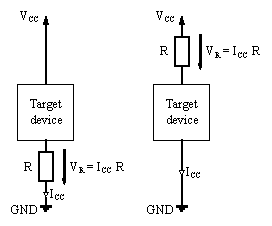
\includegraphics[width=0.5\textwidth]{figures/impl_attacks/measurement}	
		\caption{Typical measurement setup for power consumption side-channel attacks}
		\label{fig:impl_attacks:measurement}
\end{figure} 


\paragraph{Measurement Setup}
Figure~\ref{fig:impl_attacks:measurement} shows the two most typical setups for measuring the power (current) consumption of a target device. In the left setup, a (small) shunt resistor $R$\footnote{usually between 1\,$\Upomega$ and several hundred $\Upomega$} is inserted into the ground path of the target device. Since the supply current $I_{CC}$ flows through the resistor, it can be derived by measuring the voltage drop $V_R$ over $R$ as $I_{CC} = \frac{V_R}{R}$. Note that in \ac{SCA}, usually, we are not interested in the absolute value of $I_{CC}$, but rather require only a value proportional to it. Hence, in practice, one can just measure $V_R$ with a \ac{DSO} and ignore the conversion factor $R$. 

An alternative approach is to place $R$ into the $V_{CC}$ path and again measure the drop over $V_R$. Since $I_{CC}$ is the same for both paths, this approach is equivalent to measuring in the ground path (if there is only one supply voltage). However, when attaching a standard \ac{DSO} probe to measure $V_R$ in the $V_{CC}$ path, note that one obtains $V_{CC} - V_R$, i.e., the signal is \acs{DC}-shifted. Hence, one has to remove the constant \acs{DC} component by measuring \acs{AC}-coupled. Alternatively, $V_R$ can be directly measured using a so-called differential probe. 


%\subsection{Timing}

\subsection{\acl{SPA}}
\acf{SPA} is an umbrella term for side-channel attacks that work by (visually) inspecting one or a few traces. For instance, take the \ac{SAM} (Algorithm~\ref{alg:asymmetric_crypto:ln_sam}): if an adversary can distinguish squaring (SQ) and multiply (MUL), he can trivially reconstruct the secret exponent bit-by-bit. Take the example of the trace in Figure~\ref{fig:impl_attacks:spa_rsa}: The executed operation sequence is: SQ, MUL, SQ, MUL, SQ, SQ, SQ, MUL, SQ, SQ, MUL. 

\begin{figure}[h!tb]
		\center
		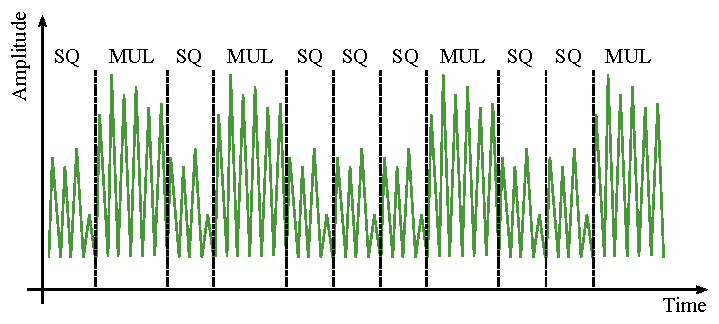
\includegraphics[width=0.7\textwidth]{figures/impl_attacks/spa_rsa}	
		\caption{\ac{SPA} of \ac{SAM} algorithm for \ac{RSA} signature}
		\label{fig:impl_attacks:spa_rsa}
\end{figure} 

\subsection{\acl{DPA}}
\label{sec:impl_attacks:dpa}
While \ac{SPA} attacks utilize larger amounts of side-channel leakage (e.g., of a long-number multiplication consuming many cycles), \acf{DPA}~\cite{dpa_kocher} can exploit tiny leakages (e.g., of a single bit being processed on a large \ac{IC}). To this end, \ac{DPA} uses statistical methods to detect the tiny leakage signal in a larger amount of (noisy) traces. The core assumption of \ac{DPA} is that the power consumption (or other side-channel signals) are slightly different if the target device processes a zero bit or a one bit. However, in contrast to \ac{SPA}, this difference does not have to be ``visible'' and further can be hidden in noise.

A typical \ac{DPA} is divided into two steps, the measurement and evaluation phase, which are described in the following.

\paragraph{Measurement}
\ac{DPA} operates on a set of $n$ traces $p_i \left( t \right)$ with $T$ sample points each (i.e., $t = 0\,\ldots\,T-1$). Each trace is the power consumption while the target device encrypts a plaintext $X_i$ (or performs another cryptographic operation) using the key $k$. In the following, when we talk about bytes (or other parts) of $x_i$, we will use the notation $X_i^0$ to for example denote byte~0 of $X_i$. If it is clear from the context that we only talk about a specific byte, we write $x_i$. The measurement phase is summarized in Algorithm~\ref{alg:impl_attacks:dpa_measure}.

\begin{algorithm}
\center
\begin{algorithmic}
\vspace{2mm}

\For{$i = 0  \ldots n-1$}
	\State Generate random, uniformly distributed plaintext $X_i$
	\State Send $X_i$ to device, device computes $enc_K \left(X_i \right)$
	\State Measure power consumption $p_i\left(t\right)$
	\State Store $p_i\left(t\right)$ and corresponding $X_i$
\EndFor

\vspace{2mm}
\end{algorithmic}
\caption{Measurement phase of a \ac{DPA}}
\label{alg:impl_attacks:dpa_measure}
\end{algorithm}

\paragraph{Evaluation}


The evaluation process (for the first byte/part $k$ of the round key) for the example of the \ac{AES} is summarized in Algorithm~\ref{alg:impl_attacks:dpa_eval}.

\begin{algorithm}[h!tb]
\center
\begin{algorithmic}
\vspace{2mm}

\State $S_{0}^{\hat{k}}\left(t\right) \gets\ $  empty set for each candidate $\hat{k}$ for $k$
\State $S_{1}^{\hat{k}}\left(t\right) \gets\ $  empty set for each candidate $\hat{k}$ for $k$
\vspace{2mm}
\For{$i = 0  \ldots n-1$}
	\vspace{1mm}
	\State Load trace $p_i\left(t\right)$ and plaintext $X_i$
	\State $x_i \gets\ $ first byte/part of $X_i$
	\vspace{1mm}
	\For{$\hat{k} = 0 \ldots 255$}
		\vspace{1mm}
		\State $b \gets S\left(x_i\,\oplus\,\hat{k}\right)$
		\If{$\mbox{LSBit}\left(b\right) = 0$}
			\State Add $p_i\left(t\right)$ to $S_{0}^{\hat{k}}$
		\Else
			\State Add $p_i\left(t\right)$ to $S_{1}^{\hat{k}}$
		\EndIf
	\EndFor
	\vspace{1mm}	
\EndFor
\vspace{2mm}
\For{$\hat{k} = 0 \ldots 255$}
	\vspace{2mm}
	\State $\overline{S}_{0}^{\hat{k}}\left(t\right) \gets \frac{1}{\left|S_{0}^{\hat{k}}\right|} \sum_{p_i \in S_{0}^{\hat{k}}}{p_i\left(t\right) }$
	\State  $\overline{S}_{1}^{\hat{k}}\left(t\right) \gets \frac{1}{\left|S_{1}^{\hat{k}}\right|} \sum_{p_i \in S_{1}^{\hat{k}}}{p_i\left(t\right) }$
	\vspace{2mm}
	\State $\mbox{DPA}^{\hat{k}}\left(t\right) \gets \overline{S}_{1}^{\hat{k}}\left(t\right) - \overline{S}_{0}^{\hat{k}}\left(t\right)$
\vspace{2mm}
\EndFor
\vspace{2mm}
\State Find $\mbox{DPA}^{\hat{k}}$ with highest peak to recover $k = \hat{k}$.

\end{algorithmic}
\caption{Evaluation phase of a \ac{DPA} for first byte of \ac{AES}}
\label{alg:impl_attacks:dpa_eval}
\end{algorithm}

\paragraph{Why \acs{DPA} works}
\ac{DPA} apparently allows to target the leakage of a single bit of a single register or memory location in a potentially very large circuit. The question arises why this approach works. The main reason is that we \emph{average} many signals, which reduces the amount of noise relatively to the signal (i.e., the leakage of a single bit). More precisely, we can write a power trace at a point in time $t_0$ as 

$$p\left(t_0\right) = p_{signal} + \mathcal{N}_{alg} + \mathcal{N}_{measure}$$

where $p_{signal}$ is the actual leakage, $\mathcal{N}_{alg}$ algorithmic noise (caused by all the parts of the circuit we do not predict), and $\mathcal{N}_{measure}$ measurement noise (i.e., physical effects in the setup etc.). Assuming $\mathcal{N}_{alg}$, $\mathcal{N}_{measure}$ are Gaussian, for $n \rightarrow \infty$, the noise vanishes and we only see the differences between $p_{signal}$ (bit = 0 and bit = 1) in the difference of means. In practice, $n \rightarrow \infty$ can mean anything between a few ten to millions or billions of traces.

\subsection{\acl{CPA}}
In a \ac{DPA}, we focus on a single bit, while we actually predict more information (e.g., 8~bit for the AES). To make use of this fact and reduce the number of required traces, \acf{CPA}~\cite{Brie04} makes use of a \emph{leakage model}---i.e., the fact that we can approximate how an internal value $b$ affects the leakage signal $p_{signal}$. Figure~\ref{fig:impl_attacks:dpa_signal} shows an example how a single byte could leak: internal values with a lower number of ones result in a lower amplitude, while more ones lead to higher values.

This leakage model is the \ac{HW} model: the side-channel signal is proportional to the \ac{HW} of the processed value, i.e., we have $p_{signal} \propto \mbox{HW} \left(b\right)$. As a reminder, $\mbox{HW} \left(b\right)$ is defined as the number of bits set to~1 in $b$. For instance, $\mbox{HW} \left(0x00\right) = 0$, $\mbox{HW}\left(0xAB\right) = \mbox{HW}\left(10101011\right) = 5$, and $\mbox{HW} \left(0xFF\right) = 8$.

\begin{figure}[h!tb]
		\center
		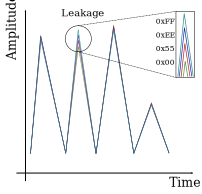
\includegraphics[width=0.4\textwidth]{figures/impl_attacks/dpa_signal}	
		\caption{Leakage of a single byte value $b$}
		\label{fig:impl_attacks:dpa_signal}
\end{figure} 

There are many other conceivable leakage models, the most prominent one being the \ac{HD} model, that assumes that the leakage depends on the \emph{previous} value $b'$ and the \emph{new} value $b$ of a register. The \ac{HD} is the number of bits that have changed between $b'$ and $b$, i.e., $\mbox{HD}\left(b',\,b\right) = \mbox{HW}\left(b'\, \oplus\,b\right)$.

In the following, we use notation based on Section~\ref{sec:impl_attacks:dpa} to explain how \ac{CPA} allows to include the leakage model into an approach similar to \ac{DPA}. Again, we have $n$ traces $p_i \left( t \right)$ with $T$ sample points each and the corresponding plaintexts $X_i$. 
Again, take the example of the \ac{AES} and assume a key candidate $\hat{k}$ for the first \ac{SBOX} with input byte $x_i$. Then, we predict the intermediate value as:

$$
b_{i,\hat{k}} \gets S\left(x_i\,\oplus\,\hat{k}\right)
$$
\vspace{-1mm}

Now, we employ our leakage model $f\left(\cdot\right)$ to convert this value into a hypothetical power consumption (e.g., using the \ac{HW} model): 

$$
h_{i,\hat{k}} = f \left(b_{i,\hat{k}}\right) \stackrel{\mbox{\tiny e.g.}}{=} \mbox{HW}\left( b_{i,\hat{k}}\right)
$$
\vspace{-1mm}

The final step is to determine the ``match'' between the predictions $h_{i,\hat{k}}$ for a key candidate and the reality of the traces $p_i \left( t \right)$. To this end, we use \emph{Pearson's correlation coefficient}~$\rho$, cf.~\cite{wiki:Pearson}. $\rho$ estimates the linear correlation between two data sets $A_i$ and $B_i$: if they are perfectly correlated, $\rho = 1$ and one data set can be written as a linear function $A_i = \alpha \cdot B_i + \beta$ of the other. If there is no correlation, $\rho = 0$. For perfectly inverse-correlated data sets, $\rho = -1$. 
In summary, keep in mind that $-1 \leq \rho \leq 1$.

In our case, one data series is the set of traces $p_i \left( t \right)$, the other one the prediction $h_{i,\hat{k}}$. Since $p_i \left( t \right)$, we compute the correlation point-wise for each time sample. However, note that $h_{i,\hat{k}}$ is not time-dependent, hence, this data series is always the same for all $t$.

Thus, given a key candidate $\hat{k}$, we obtain:

$$
\rho_{\hat{k}}\left(t\right) = \frac{\sum\limits_{i = 0}^{n-1} {\left( h_{i,\hat{k}} - \overline{h}_{\hat{k}}  \right) \cdot \left( p_{i}\left(t\right) - \overline{p}\left(t\right) \right)} }   {\sqrt{\sum\limits_{i = 0}^{n-1} {\left( h_{i,\hat{k}} - \overline{h}_{\hat{k}}\right)^2}\ \cdot \ \sum\limits_{i = 0}^{n-1} {\left( p_{i}\left(t\right) - \overline{p}\left(t\right)\right)^2 }   }} = \frac{\mbox{cov} \left(h_{i,\hat{k}}, p_i\left(t\right)\right)}{\sqrt{\mbox{var}\left(h_{i,\hat{k}}\right) \cdot \mbox{var}\left(p_i\left(t\right)\right)}}
$$

$\rho_{\hat{k}}\left(t\right)$ is the equivalent to the difference-of-means curve $\mbox{DPA}^{\hat{k}}\left(t\right)$ in a \ac{DPA}---the correlation with the highest peak identifies the correct key candidate.

\paragraph{Rules of Thumb} 
In contrast to \ac{DPA}, where the value of a peak in the difference-of-means is hard to predict, \ac{CPA} is normalized to the range $-1 \leq \rho \leq 1$, which makes it easier to define what a \emph{significant} correlation is. \cite{MangardOP_DPABook_07} provides several ``rules of thumb'' for the correlation coefficient.
First, for $n$ traces, the expected ``noise level'' $\rho$ is

$$
\rho_{noise} = \frac{4}{\sqrt{n}}
$$

That means that any correlation $\leq \rho_{noise}$ is essentially meaningless and not significant. This formula reflects the fact that for more traces, it is possible to identify smaller correlations. The second rule of thumb allows to estimate the minimum number of required traces $n_{min}$ to unambiguously extract a key (with very high probability) when the respective correlation for the correct key $\rho_{key}$ is known (e.g., from prior experiments). 

$$
n_{min} = \frac{28}{\rho_{key}^2}
$$

This formula only holds for $\rho_{key} \leq 0.2$. To give an example: Assume after $n = 2000$ traces, we get $\rho_{key} = 0.1$. Clearly, this correlation is significant since $\rho_{noise} = \nicefrac{4}{\sqrt{2000}} = 0.089$. However, to be able to unambiguously extract the key with that correlation, $n_{min} = \nicefrac{28}{0.1^2} = 2800$~traces would be required.

\section{Countermeasures}
Protecting against \ac{SCA} has been an active area of research since the initial discovery around~2000. Hence, we can only look at a small selection of countermeasures in this section. A deeper survey for block ciphers is for example given in~\cite{prouff_ches2013}. Countermeasures to directly thwart \ac{SCA} can be realized on two dimensions (and a combination of them): the amplitude of the leakage and the timing. In addition, countermeasures on the system level can be taken to limit the consequences of successful \ac{SCA}, rather than preventing the actual attack. We will consider examples for all three approaches in this section.

\subsection{Amplitude-based Countermeasures}
The \ac{SNR} determines the success rate of a side-channel attack---the lower the \ac{SNR}, the more measurements will be needed in general. 

\paragraph{Balanced Logic Styles}
A first way to reduce the \ac{SNR} is to reduce the power of the leakage signal by balancing the power consumption. As a simple example, assume all results are computed on differential signals (i.e., a bit $a$ and the complement $\overline{a}$ are always used at the same time). Then, ideally, the leakage should vanish: For example, assuming a \ac{HW} model, we would always observe $\mbox{HW}\left(a\right) + \mbox{HW}\left(\overline{a}\right) = \mbox{const}$, independent of the value of $a$. There is a variety of such balanced logic styles\footnote{For a good overview, cf.~e.g.~\url{https://www.cosic.esat.kuleuven.be/ecrypt/courses/albena11/slides/amir_moradi_secure_logic_styles.pdf}}. However, due to various effects in real \acp{IC} (different routing delays, capacitance, process variations in general), the countermeasures can never fully remove the side-channel leakage. Yet, they help to make \ac{SCA}, especially in combination with other countermeasures, much more difficult.

Another (rather obvious) example for a countermeasure based on reducing the information in the signal is protection against \ac{SPA}, for example for \ac{SAM}-like algorithms. Instead of using a specific implementation for squaring that produces a distinguishable pattern, multiplication can be used for both operations. However, a squaring realized with multiplication may still be recognizable, e.g., because of different memory access patterns. One solution is to use a Square-and-Multiply-always approach, where the result of the multiplication is discarded if the current exponent bit is zero. Other, more refined algorithms like the Montgomery ladder~\cite{montgomery1987speeding} ensure that the same number of squares and multiplications is executed (independent of the exponent) by using two result registers. Note however that \ac{SPA}-protected algorithms are usually still vulnerable to \ac{DPA}.

\paragraph{Noise Generation}
Reducing the \ac{SNR} can alternatively be achieved by increasing the amount of noise. A hardware or software-based noise generator can be used for this purpose, but it should be noted that averaging will allow the adversary to remove this noise again. In other words, noise generation (when used as the only countermeasure) will only increase the number of required traces. However, in combination with other countermeasures (e.g.~randomized timing, see below), it can severely impede \ac{SCA}, for example, because an adversary can no longer re-align traces in time based on signal patterns.

%% Masking
\paragraph{Masking}
Instead of introducing uncorrelated noise or reducing the leakage, \emph{masking} fully randomizes all sensitive internal variables by internally generating a fresh, random mask for each execution of an algorithm. Then, the device only leaks the masked values, which an adversary cannot predict since the mask never ``leaves'' the device. An early description of such a method can e.g.~be found in~\cite{chari1999towards}.

The general idea is to combine the sensitive value $x$ with a random mask $m$, e.g., using \verb+XOR+. Then, the device performs all computations on $x \oplus m$, and unmasks the result before outputting. For operations that are linear with respect to \verb+XOR+ (e.g., \verb+XOR+ing a round key), applying masking is trivial, since for example $\left(x \oplus m\right) \oplus k = \left(x \oplus k\right) \oplus m$.
%
For non-linear components, e.g., an \ac{SBOX} $S$, masking requires to generate a new, masked \ac{SBOX} $S_m$ such that $S_m\left(x \oplus m\right) = S\left(x\right) \oplus m$. In general, the masked \ac{SBOX} depends on $m$ and has to be generated on-the-fly or precomputed for all $m$. However, for specific cases, e.g., the \ac{AES} \ac{SBOX}, algebraic properties can be utilized for more efficient realization~\cite{oswald2005side,canright2008very}.
%
Masking can be understood as being based on secret sharing and multiparty computation, which has lead to newer developments like so-called \emph{threshold implementations}~\cite{nikova2006threshold}.

From the attacker's point of view, masking schemes can be attacked in various ways: first of all, if the random mask $m$ is biased, attacks may still succeed with a larger number of traces. Furthermore, \emph{higher-order} \ac{SCA} (where multiple sample points are combined to exploit combined leakage of sensitive value and mask) allows to mount \ac{DPA} or \ac{CPA} also for masked implementations~\cite{oswald2006practical}.

\subsection{Timing-based Countermeasures}
In contrast to amplitude-based approaches, timing-based countermeasures lower the \ac{SNR} by spreading the leakage over multiple clock cycles. Again, there are various ways to achieve this goal: 
first, the clock signal can be made unstable on purpose, or even randomly frequency-modulated so that a targeted operation is executed at different points in time for subsequent executions of the algorithm. It should be noted that an adversary may be able to re-align a set of traces, e.g., by extracting the peaks in the traces, using pattern matching, or \acs{FM}-demodulating the traces.

Instead of manipulating the shape of the clock signal, dummy operations (or dummy cycles) can be added to the control flow to ensure that a target intermediate value is handled in different clock cycles for different executions. The dummy operations should obviously be indistinguishable from ``real'' operations, otherwise the adversary may be able to remove them, again using pattern matching techniques. 

A slightly more algorithm-specific approach with similar ideas is to randomly change the order of operations (``shuffling''), e.g., the \ac{SBOX} instances of the \ac{AES}. Of course, this is only possible for operations that have no dependency (e.g., \acp{SBOX} applied byte-wise) or that are commutative (e.g., when \verb+XOR+ing or adding several values). A comprehensive discussion can for example be found in~\cite{veyrat2012shuffling}.

It should be noted that timing-based countermeasures generally linearly reduce the attack efficiency, i.e., if a target sample is spread over $\tau$ samples, then the efficiency decreases by a factor of $\tau$. However, by averaging (integrating) all potential target samples (in the simplest case summing $\tau$ samples), this factor becomes $\sqrt{\tau}$. Hence, in practice, protecting an implementation by time randomization alone would require a very large parameter $\tau$. Therefore, they are usually used in combination with other countermeasures.

As a final note, an equally (or potentially even more) important aspect is the protection against timing attacks that exploit secret-dependent runtime variations. It is mandatory that the cryptographic algorithm itself has constant runtime for any combination of inputs (i.e., usually key and plaintext). Amongst others, bitslicing (Section~\ref{sec:symmetric_crypto:bitslicing}) can be used to achieve this goal. The timing randomization then is applied on top of the constant-runtime algorithm, e.g., by inserting dummy cycles. The entropy for the randomization must be independent of the inputs to the algorithm---otherwise, if input data is used to derive ``randomness'' for countermeasures, a trivial timing vulnerability may be inserted into the algorithm. 

\subsection{System Level Countermeasures}
First and foremost, a central countermeasure on the system level is to \emph{diversify} keys, especially for devices that the adversary may get physical access to. This implies that every device gets a unique key---if an adversary manages to extract this key, only one specific device is affected. 
%
What happens when this principle is not followed can be see by the example of a digital locking system~\cite{crypto_paper_sv,Oswald13_1}. In this case, a symmetric master key was present in every locking cylinder of a complete installation (a very large building complex). By attacking a single lock, the adversary can create a device to unlock any door and access any room in the entire installation. 

This is a typical example of a \ac{SPOF}, where a single successful attack has far-reaching consequences. Incidentally, note that attacks on the hardware level are only one of many ways such a master key could be leaked. Other possibilities include insiders (e.g., displeased or bribed employees), network-level attacks and rootkits (key is stored on a vulnerable computer), or unfortunate accidents (backup coy of key is stored on a decommissioned harddrive).

In contrary, for systems with proper key diversification, this problem can be largely avoided, although in general there will likely remain some valuable secrets, yet these are handled in the backend and can be protected by a variety of countermeasures. For example, in the case of a public transport card, proper key diversification ensured that a successful \ac{SCA} did not scale to the compromise of the entire system, but only affected the targeted card~\cite{OswaldPhD13}.

Note that in other cases, e.g., the protection or encryption of device firmware and bitstreams~\cite{Moradi13,Strobel15,Swierczynski14,actelSca,SCAV4V5}, key diversification is not always applicable. Even if keys are diversified, an adversary who solely wants to extract \ac{IP} (e.g., to clone a device) succeeds if he can break the protection on one single device. In these case, strong classical countermeasures are hence of particular importance.

There is a variety of other possible approaches, some implemented on the actual device, others in the backend. To name a few examples: The backend system of a locking system could check for inconsistent access attempts (e.g., two distant doors were accessed approximately at the same time by the same user) to detect cloned tokens. The same applies to payment systems, where shadow accounts can be used to verify that the balance spent with a particular payment card agrees with the  amount charged by the user. In general, devices which are suspected to have been compromised can be blocked. 
In addition, implementation attacks can be detected (or mitigated) on the side of the device, e.g., by blocking suspicious activities like the acquisition of many side-channel traces (attempt or rate limiting). 

In general, system-level countermeasures strongly depend on the particular application and should hence be seen as a ``second line of defense'', should the traditional countermeasures be overcome.

%---------------------------------------------------------------------






%#####################################################################
%                       Bibliography
%#####################################################################
\addcontentsline{toc}{chapter}{Bibliography}
\bibliographystyle{alpha} % plain or alpha
\bibliography{literature}

%#####################################################################
%                       List of Abbreviations
%#####################################################################
\addcontentsline{toc}{chapter}{List of Abbreviations}
\chapter*{List of Abbreviations}

\begin{acronym}
 \setlength{\itemsep}{0.2em}
 \acro{3DES}{Triple DES}
 \acro{AA}{Active Authentication}
 \acro{AC}{Alternating Current}
 \acro{ADC}{Analog to Digital Converter}
 \acro{ACK}{Acknowledgement}
 \acro{AES}{Advanced Encryption Standard}
 \acro{AID}{Application Identifier}
 \acro{ANF}{Algebraic Normal Form}
 \acro{APDU}{Application Protocol Data Unit}
 \acro{API}{Application Programming Interface}
 \acro{ASCII}{American Standard Code for Information Interchange}
 \acro{ASCA}{Algebraic Side-Channel Analysis}
 \acro{ASK}{Amplitude-Shift Keying}
 \acro{ASIC}{Application Specific Integrated Circuit}
 \acro{ATQA}{Answer To Request A}
 \acro{ATR}{Answer To Reset}
 \acro{ATS}{Answer To Select}
 \acro{BAC}{Basic Access Control}
 \acro{BPSK}{Binary Phase Shift Keying}
 %\acro{BSI}{Bundesamt für Sicherheit in der Informationstechnik}
 \acro{CBC}{Cipher Block Chaining}
 \acro{CC}{Common Criteria}
 \acro{CCA}{Canonical Correlation Analysis}
 \acro{CHES}{Cryptographic Hardware and Embedded Systems}
 \acro{CIA}{Combined Implementation Attacks} 
 \acro{CL}{Cascade Level}
 \acro{CMRR}{Common Mode Rejection Ratio}
 \acro{CMTF}{Combined Masking in Tower Fields}
 \acro{CMOS}{Complementary Metal Oxide Semiconductor}
 \acro{CNF}{Conjunctive Normal Form}
 \acro{COPACOBANA}{Cost-Optimized Parallel Code Breaker and Analyzer}
 \acro{COSY}{Communication Security}
 \acro{CPA}{Correlation Power Analysis}
 \acro{CPU}{Central Processing Unit}
 \acro{CRC}{Cyclic Redundancy Check}
 \acro{CRT}{Chinese Remainder Theorem}
 \acro{CTR}{Counter \acroextra{(mode of operation)}}
 \acro{DAC}{Digital-Analog Converter}
 \acro{DECT}{Digital Enhanced Cordless Telecommunications}
 \acro{DES}{Data Encryption Standard}
 \acro{DEMA}{Differential Electro-Magnetic Analysis}
 \acro{DC}{Direct Current}
 \acro{DCM} {Digital Clock Manager}
 \acro{DFA}{Differential Frequency Analysis}
 \acro{DFT}{Discrete Fourier Transform}
 \acro{DoM}{Difference of Means}
 \acro{DoS}{Denial-of-Service}
 \acro{DIP}{Dual Inline Package}
 \acro{DIMM}{Dual In Line Memory Modules}
 \acro{DNF}{Disjunctive Normal Form}
 \acro{DOM}{Difference-of-Means}
 \acro{DPA}{Differential Power Analysis}
 \acro{DRAM}{Dynamic Random Access Memory}
 \acro{DSO}{Digital Storage Oscilloscope}
 \acro{DSP}{Digital Signal Processing}
 \acro{DST}{Digital Signature Transponder}
 \acro{DTW}{Dynamic Time Warping}
 \acro{DUT}{Device Under Test}
 \acroplural{DUT}[DUTs]{Devices Under Test}
 \acro{DVB-T}{Digital Video Broadcasting -- Terrestrial}
 \acro{EAC}{Extended Access Control}
 \acro{ECB}{Electronic Code Book}
 \acro{ECC}{Elliptic Curve Cryptography}
 \acro{ECU}{Electronic Control Unit}
 \acro{ECDLP}{Elliptic Curve Discrete Logarithm Problem}
 \acro{ECMA}{European Computer Manufacturers Association}
 \acro{EDE}{Encrypt-Decrypt-Encrypt \acroextra{(mode of operation)}}
 \acro{EEPROM}{Electrically Erasable Programmable Read-Only Memory}
 \acro{EM}{Electro-Magnetic}
 \acro{EMC}{Electro-Magnetic Compatibility}
 \acro{EMSEC}{Embedded Security}
 \acro{EOC}{End Of Communication}
 \acro{EOF}{End Of File}
 \acro{ePass}{Electronic Passport}
 \acro{EPC}{Electronic Product Code}
 \acro{EU}{European Union}
 \acro{FDT}{Frame Delay Time}
 \acro{FF}{Flip Flop}
 \acro{FFT}{Fast Fourier Transform}
 \acro{FI}{Fault Injection}
 \acro{FIB}{Focused Ion Beam}
 \acro{FIFO}{First In First Out \acroextra{(memory)}}
 \acro{FIPS}{Federal Information Processing Standard}
 \acro{FIR}{Finite Impulse Response} 
 \acro{FIT}{Faculty of Information Technology}
 \acro{FM}{Frequency Modulation}
 \acro{FPGA}{Field Programmable Gate Array}
 \acro{FRAM}{Ferroelectric RAM}
 \acro{FSM}{Finite-State Machine}
 \acro{FSK}{Frequency Shift Keying}
 \acro{GIAnT}{Generic Implementation Analysis Toolkit}
 \acro{GND}{Ground}
 \acro{GNFS}{General Number Field Sieve}
 \acro{GUI}{Graphical User Interface}
 \acro{GPIO}{General Purpose I/O}
 \acro{GPL}{GNU General Public License}
 \acro{GPS}{Global Positioning System}
 \acro{GSM}{Global System for Mobile Communications}
 \acro{HAC}{Handbook of Applied Cryptography}
 \acro{HD}{Hamming Distance}
 \acro{HDL}{Hardware Description Language}
 \acro{HF}{High Frequency}
 \acro{HGI}{Horst Görtz Institute for IT Security}
 \acro{HID}{Human Interface Device}
 \acro{HLTA}{HaLT type A}
 \acro{HMAC}{Hash-based Message Authentication Code}
 \acro{HOTP}{HMAC-based One Time Password}
 \acro{HVSP}{High Voltage Serial Programming} 
 \acro{HVG}{High Voltage Generator}
 \acro{HW}{Hamming Weight}
 \acro{ICAO}{International Civil Aviation Organization}
 \acro{IC}{Integrated Circuit}
 \acro{ICC}{Integrated Circuit Card}
 \acro{ID}{Identifier}
 \acro{IDE}{Integrated Development Environment}
 \acro{IFD}{Interface Device}
 \acro{IGBT}{Insulated Gate Bipolar Transistor}
 \acro{IoT}{Internet of Things}
 \acro{ISO}{International Organization for Standardization}
 \acro{ISM}{Industrial, Scientific, and Medical \acroextra{(frequencies)}}
 \acro{IFF}{Identify Friend or Foe}
 \acro{IIR}{Infinite Impulse Response}
 \acro{IP}{Intellectual Property}
 \acro{ISR}{Interrupt Service Routine}
 \acro{ISP}{In-System Programming}
 \acro{IV}{Initialization Vector}
 \acro{JTAG}{Joint Test Action Group}
 \acro{KDF}{Key Derivation Function}
 \acro{LAN}{Local Area Network}
 \acro{LED}{Light-Emitting Diode}
 \acro{LF}{Low Frequency}
 \acro{LFSR}{Linear Feedback Shift Register}
 \acro{LIW}{Listening Window}
 \acro{LSB}{Least Significant Bit}
 \acro{LSByte}{Least Significant Byte}
 \acro{LUT}{Look-Up Table}
 \acro{MAC}{Message Authentication Code}
 \acro{MF}{Medium Frequency}
 \acro{MIA}{Mutual Information Analysis}
 \acro{MITM}{Man-In-The-Middle}
 \acro{MOSFET}{Metal-Oxide Semiconductor Field-Effect Transistor}
 \acro{MRZ}{Machine Readable Zone}
 \acro{MRTD}{Machine Readable Travel Document}
 \acro{MSB}{Most Significant Bit}
 \acro{MSByte}{Most Significant Byte}
 \acro{muC}[$\mathrm{\upmu C}$]{Microcontroller}
 \acro{nPA}{New German ID Card}
 \acro{NACK}{Negative Acknowledgment}
 \acro{NDA}{Non-Disclosure Agreement}
 \acro{NIST}{National Institute of Standards and Technology}
 \acro{NLFSR}{Non-Linear Feedback Shift Register}
 \acro{NLF}{Non-Linear Function}
 \acro{NFC}{Near Field Communication}
 \acro{NRZ}{Non-Return-to-Zero \acroextra{(encoding)}}
 \acro{NOP}{No Operation}
 \acro{NVM}{Non-Volatile Memory}
 \acro{OATH}{Initiative of Open Authentication}
 \acro{OOK}{On-Off-Keying}
 \acro{OP}{Operational Amplifier}
 \acro{OS}{Operating System}
 \acro{OTP}{One-Time Password}
 \acro{PA}{Passive Authentication}
 \acro{PACE}{Password Authenticated Connection Establishment}
 \acro{PC}{Personal Computer}
 \acro{PCA}{Principal Component Analysis}
 \acro{PCB}{Printed Circuit Board}
 \acro{PCD}{Proximity Coupling Device}
 \acro{PEA}{Photonic Emission Analysis}
 %\acro{PhD}{Patiently hoping for a Degree}
 \acro{PICC}{Proximity Integrated Circuit Card}
 \acro{PIT}{Programmable Identification Transponder}
 \acro{PKI}{Public Key Infrastructure}
 \acro{PLL} {Phase Locked Loop}
 \acro{PMS}{Perfectly Masked Squaring}
 \acro{PMM}{Perfectly Masked Multiplication}
 \acro{PPC}{Pulse Pause Coding}
 \acro{PPS}{Protocol and Parameter Selection}
 \acro{PPSR}{Protocol and Parameter Selection Request}
 \acro{PRN}{Pseudo-Random Number}
 \acro{PRNG}{Pseudo-Random Number Generator}
 \acro{PS}{Passive Serial \acroextra{(mode)}}
 \acro{PSK}{Phase Shift Keying}
 \acro{RADAR}{Radio Detection And Ranging}
 \acro{RAM}{Random Access Memory}
 \acro{RATS}{Request for Answer To Select}
 \acro{REQA}{REQuest type A}
 \acro{RISC}{Reduced Instruction Set Computer}
 \acro{RF}{Radio Frequency}
 \acro{RFID}{Radio Frequency IDentification}
 \acro{RGT}{Request Guard Time}
 \acro{RKE}{Remote Keyless Entry}
 \acro{RNG}{Random Number Generator}
 \acro{ROM}{Read Only Memory}
 \acro{RSA}{Rivest Shamir and Adleman \acroextra{(cryptosystem)}}
 \acro{RTF}{Reader Talks First}
 \acro{RUB}{Ruhr-University Bochum}
 \acro{SAK}{Select AcKnowledge}
 \acro{SAM}{Square-and-Multiply}
 \acro{SBOX}[S-Box]{Substitution Box}
 \acrodefplural{SBOX}[S-Boxes]{Substitution Boxes}
 \acro{SCA}{Side-Channel Analysis}
 \acro{SDK}{Software Development Kit}
 \acro{SDR}{Software-Defined Radio}
 \acro{SECT}{Security Transponder}
 \acro{SEM}{Scanning Electron Microscopy}
 \acro{SNR}{Signal to Noise Ratio}
 \acro{SHA}{Secure Hash Algorithm}
 \acro{SHA-1}{Secure Hash Algorithm 1}
 \acro{SMA}{SubMiniature version A \acroextra{(connector)}}
 \acro{SQL}{Structured Query Language}
 \acro{SOF}{Start Of Frame}
 \acro{SOIC}{Small-Outline Integrated Circuit}
 \acro{SPA}{Simple Power Analysis}
 \acro{SPN}{Substitution-Permutation Network}
 \acro{SPOF}{Single Point of Failure}
 \acro{SRAM}{Static Random Access Memory}
 \acro{TA}{Template Attack}
 \acro{TEM}{Transmission Electron Microscopy}
 \acro{TLU}{Table Look Up}
 \acro{TTF}{Tag Talks First}
 \acro{TMTO}{Time-Memory Tradeoff}
 \acro{TMDTO}{Time-Memory-Data Tradeoff}
 \acro{TMM}{Transformed Multiplicative Masking}
 \acro{TNR}{Trace-to-Noise Ratio}
 \acro{TWI}{Two Wire Interface}
 \acro{SOC}{Start Of Communication}
 \acro{SHF}{Superhigh Frequency}
 \acro{SPI}{Serial Peripheral Interace}
 \acro{UC}[$\mu$C]{Microcontroller}
 \acro{UHF}{Ultra High Frequency}
 \acro{UID}{Unique Identifier} 
 \acro{UMTS}{Universal Mobile Telecommunications System}
 \acro{USB}{Universal Serial Bus}
 \acro{USRP}{Universal Software Radio Peripheral}
 \acro{USRP2}{Universal Software Radio Peripheral (version 2)}
 \acro{UVC} [UV-C] {Ultraviolet-C \acroextra{(light)}}
 \acro{VCP}{Virtual COM Port}
 \acro{VHF}{Very High Frequency}
 \acro{VLF}{Very Low Frequency}
 \acro{VHDL}{VHSIC (Very High Speed Integrated Circuit) Hardware Description Language}
 \acro{WLAN}{Wireless Local Area Network}
 \acro{WUPA}{Wake-UP A}
 \acro{XOR}{Exclusive OR}
\end{acronym}


%#####################################################################
%                          List of Figures
%#####################################################################
\addcontentsline{toc}{chapter}{List of Figures}
\listoffigures

%#####################################################################
%                          List of Tables
%#####################################################################
\addcontentsline{toc}{chapter}{List of Tables}
\listoftables

%#####################################################################
%                            LaTeX ends
%#####################################################################
\end{document}
